\chapter{Methylamine survey in Orion-KL
\label{chap:Orion-KL}}

In this chapter, we report the tentatively detection CH$_{3}$NH$_{2}$ in Orion-KL.

\section{Observation data}
We analyzed 2 ALMA archival data. First we used Cycle 2 data (ADS/JAO.ALMA\#2013.1.00553.S, 
\cite{Pagani+2017}) 
We also employed the ALMA Science Verification (SV) data (ADS/JAO.ALMA\#2011.0.00009.SV) 
at band 6 to fill up the missing frequency coverage of Cycle 2 data. 
\renewcommand{\arraystretch}{1.5}
\begin{table}[htb]
\begin{center}
  \caption{Summary of Observations}
  \label{tab:Obs_Ori}
{\scriptsize
  \begin{tabular}{lllllll} \hline \hline
 & Window & Frequency range & FWHM & PA \\
Date & (spw)  & (GHz) & (arcsec) & (degree) \\ \hline 
29--30 December 2014&1 & 215.145--216.087 & 1.8 $\times$1.1 & 86 \\
&2 & 216.342--217.279 & 1.8 $\times$1.1 & 84 \\
&3 & 217.273--218.211 & 2.2 $\times$1.0 & 102 \\
&4 & 218.204--219.141 & 2.2 $\times$1.0 & 102 \\
&5 & 219.127--220.064 & 1.9 $\times$1.0 & 95 \\
&6 & 219.784--220.721 & 1.8 $\times$1.0  & 95 \\
&7 & 229.757--230.694 & 1.4 $\times$0.8 & 80 \\
&8 & 230.699--231.636 & 2.1 $\times$0.9 & 102 \\
&9 & 232.238--233.175 & 1.6 $\times$1.0 & 80 \\
&10 & 233.470--234.422 & 1.6 $\times$0.8 & 90 \\
&11 & 235.084--236.021 & 1.7 $\times$0.9 & 95 \\
&12 & 236.267--237.206 & 1.6 $\times$0.9 & 87 \\
&13 & 244.834--245.771 & 1.6 $\times$0.9 & 79 \\
&14 & 245.773--246.710 & 1.6 $\times$0.9 & 79 \\
&15 & 250.154--251.091 & 1.5 $\times$0.9 & 88 \\
&16 & 251.079--252.016 & 1.3 $\times$0.8 & 86 \\ \hline
20 January 2012 & 0--16 & 213.715--246.627& 1.8$\times$1.3 & -1  \\ \hline
  \end{tabular}
  }
\end{center}
\end{table}
Details of each data are summarized in Table \ref{tab:Obs_Ori}.

Cycle 2 data cube was already calibrated by observers and the reduced data are available on 
the Internet\footnote{http://cdsarc.u-strasbg.fr/viz-bin/qcat?J/A+A/604/A32}.
Since the SV data contained not only line emission but continuum emission, 
we subtracted continuum emission statistically by the method described in Section \ref{sec:Statcont}.

In addition, we used Common Astronomy Software Applications (CASA) software \citep{McMullin+2007} 
during the procedure to analyze observational data.

\newpage
\section{Analysis}
\subsection{Reduction of SV data}
\label{sec:Statcont}

With the advent of highly sensitive facilities such as ALMA, the spectral lines which were hindered 
by the noise level with previous telescope can now be detected.
Most of these line-rich sources including hot cores are associated with detectable continuum emission.
In the analysis of molecular emission lines, the determination and the subtraction of this continuum 
emission is an essential, but difficult task. 
Therefore, we improved the method devised in \citet{Sanchez-Monge+2017} and deduced continuum subtraction 
in the observed UV domain (the raw visibilities measured by the interferometer).
We introduce the manner and results in this section.

\subsubsection*{Determination of the continuum level}
The determination of the continuum emission level of astronomical sources observed in a spectral line 
observing mode is based on the identification of channels free of line emission, i.e. line-free channels.

First, we obtain the spectra for which we want to estimate the continuum level.  
In the case of Orion-KL, many molecular emission exist in Hot core
(RA$_{J2000}: 05^{\rm{h}}35^{\rm{m}}14^{\rm{s}}.580$, Dec$_{J2000}:-05^{\circ}22'31''.029$) or 
Compact ridge(RA$_{J2000}: 05^{\rm{h}}35^{\rm{m}}14^{\rm{s}}.2775$, Dec$_{J2000}:-05^{\circ}22'30''.776$), 
so we extracted spectra from circular regions with a diameter of 1''.0  with the coordinates indicated by 
\citet{Hirota+2015} as the center.
The peak of the distribution of the intensity values is determined with a Gaussian fit 
when assuming the Gaussian random error resulting in an estimate of the mean value $E$ 
and the standard deviation $\sigma$. 
The width is small in case of pixels with little or no line emission, but for line contaminated 
regions the distribution becomes broader and the exact location of the peak more uncertain. 
Therefore, we set the range of the Gaussian fitting from 0 to 1/3 of the peak intensity in line contaminated side,
and calculated the mean value $E$ and the standard deviation $\sigma$.

\begin{figure}[htbp] 
\begin{center}
%\begin{minipage}{0.98\textwidth} 
%\begin{center}
%%%% ここから
%\begin{minipage}{0.48\textwidth}
%\begin{center}
%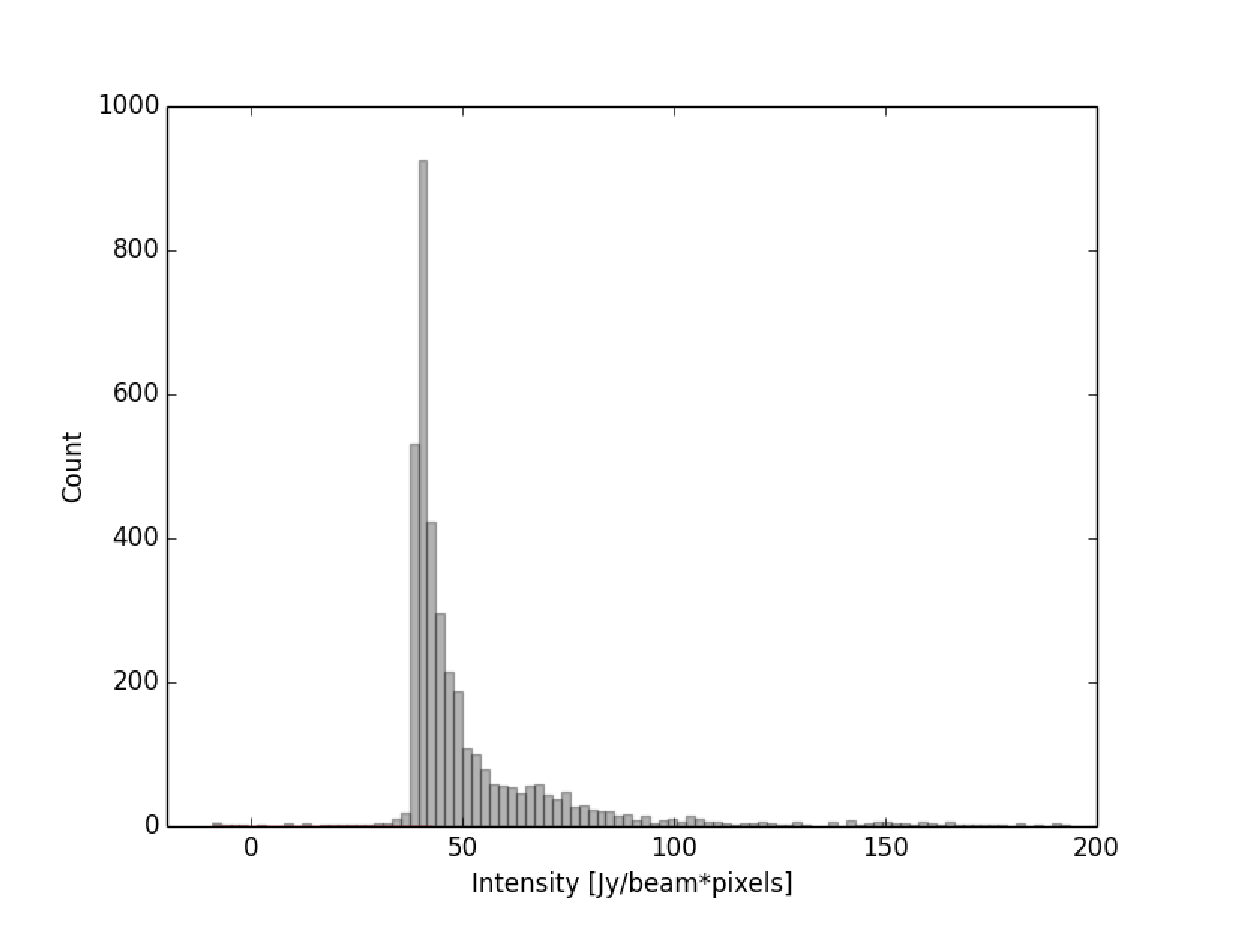
\includegraphics[width=0.98\textwidth]{OrionKL/ex_histogram.eps}
%\\(a) 左の図の説明
%\end{center}
%\end{minipage}
%\begin{minipage}{0.48\textwidth}
%\begin{center}
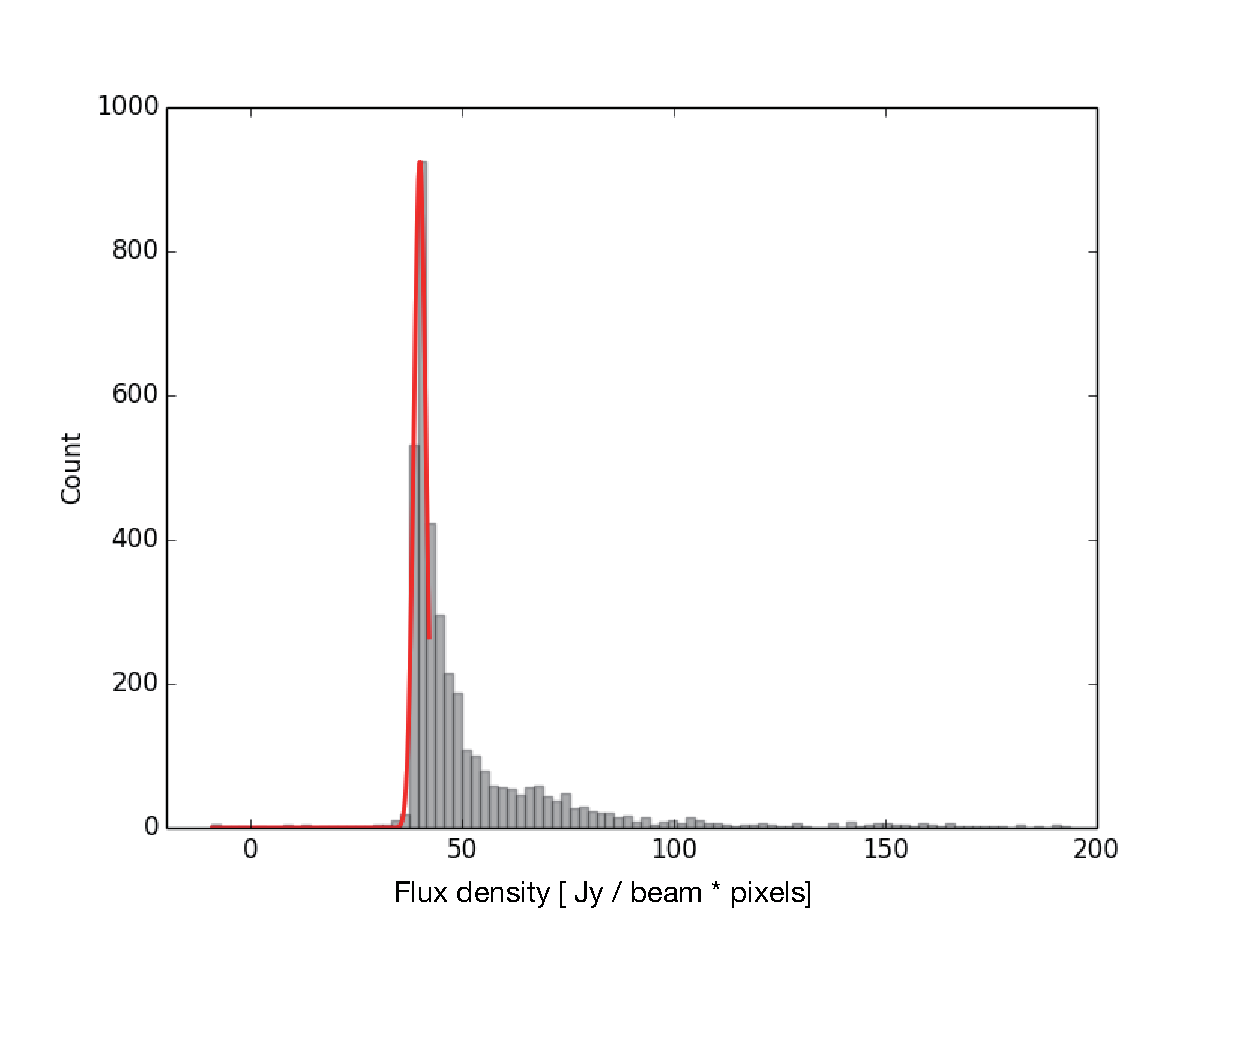
\includegraphics[width=0.8\textwidth]{OrionKL/ex_histogram_fit.eps}
%\\(b) 右の図の説明
%\end{center}
%\end{minipage}
%\end{center}
%\end{minipage}
\caption{Schematic description of the process of determination of the continuum level toward Orion-KL: 
shown are the flux distributions of Hot core (histogram) with the resulting fit overlaid (red line).}
\end{center}
\end{figure}

\newpage

\subsubsection*{Imaging line cubes}
Subsequently, the part of the distribution within $E - 3\sigma$ is defined as line-free channels.
Hot core and Compact ridges have different spectrums because of the disparate chemical composition, 
so we determined the line-free channels individually and subtracted the continuum
in the UV domain by CASA task {\sc uvcontsub} with channels common to the two regions.
After the continuum subtraction, line cubes of Orion-KL were made using the CASA task {\sc clean}.

Figure \ref{SVspec} shows examples of difference spectrum towards Hot core. 
It can be confirmed that the continuum subtraction has succeeded.

\begin{figure}[htbp]
  \centering
  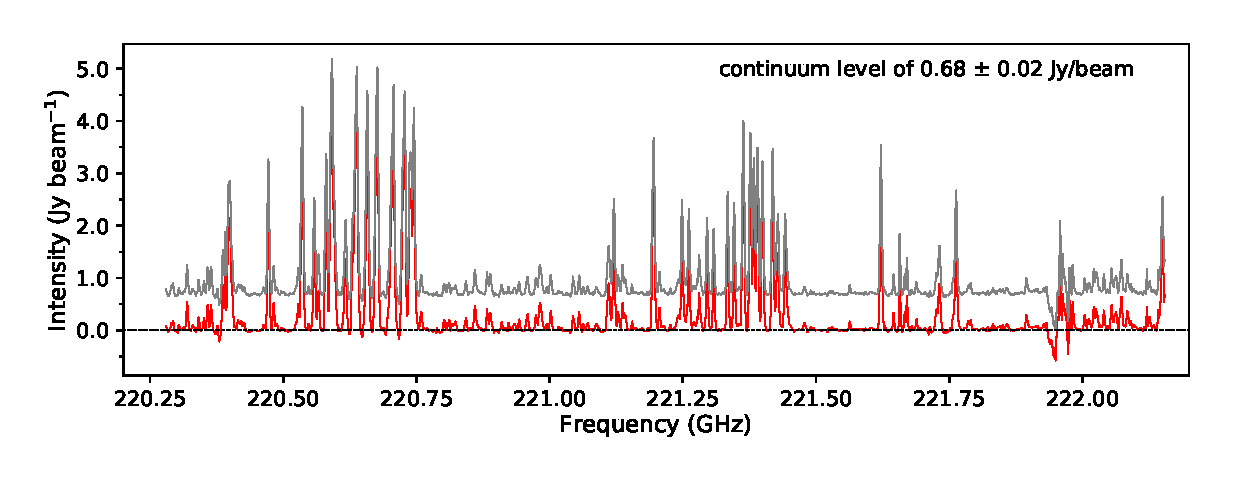
\includegraphics[width=0.98\textwidth]{OrionKL/spec_spw2.eps}
  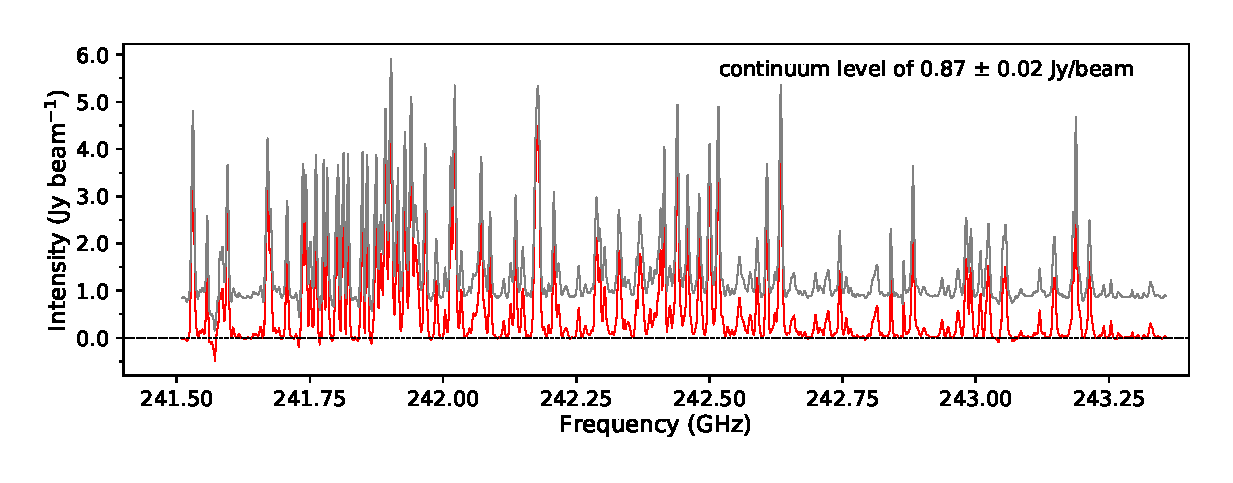
\includegraphics[width=0.98\textwidth]{OrionKL/spec_spw13.eps}
  \caption{The original spectra (gray) and continuum-subtracted spectra (red) towards Hot core. 
  The dotted line represents the base line (0 level). The continuum emission level subtracted to the original spectra, 
  together with its uncertainty, is listed in the upper right part of each panel.}
  \label{SVspec}
\end{figure}


\newpage
\subsection{Line identification}
In order to find out where common signals exist, we drew integrated intensity maps 
using CASA task {\sc immoment}. The integrated velocity range is 3.0-12.0 km s$^{-1}$, corresponding to
typical velocity component of Hot core (4.8-6 km s$^{-1}$) and that of Compact ridge 
(7.2-9.6~km~s$^{-1}$) \citep{Feng+2015}.
Spectroscopic data of CH$_3$NH$_2$ are provided by \citet{Motiyenko+2014} and 
JPL Molecular Spectroscopy catalog\footnote{http://spec.jpl.nasa.gov}.

Then, since emission at the center of Hot core were found in most of integrated intensity maps, 
we extracted spectrum for transitions with no line blending around $\pm$2 km~s$^{-1}$ from Hot core.
Possible line blending ($E_{\mathrm{u}} < 500\, \mathrm{K}$) with CH$_{3}$NH$_{2}$ was investigated by JPL database, 
the Cologne database for molecular spectroscopy (CDMS)\footnote{http://www.astro.uni-koeln.de/cdms/}, 
and Splatalogue\footnote{http://www.splalogue.net/}. 

Subsequently, we estimated the systemic velocity and the line width of 217.758~GHz line, 
reported by \citet{Pagani+2017}, which does not seem contaminated by other molecular lines.
At last, using these value, we obtained the integrated intensity of 6~transitions described in 
Table \ref{tab:MAOri} by the Gaussian fitting.


\newpage
\section{Results}
%\subsection{Transitions}
The data obtained for CH$_{3}$NH$_{2}$ are summarized in Table \ref{tab:MAOri}.
Here the rest frequencies, $S\mu^2$, the upper state energy ($E_{\mathrm{u}}$), the quantum numbers,
the peak brightness temperature, the systemic velocity (V$_{\mathrm{LSR}}$) , and noise level are given.
Out of 32 predicted transitions ($S\mu^2 > 25\,\mathrm{D^2}$ and $E_{\mathrm{u}} < 200 \,\mathrm{K}$) 
in our observational frequency range, 6 were probably identified in this data set, and are reported in
Table \ref{tab:MAOri}. The remaining 18 CH$_{3}$NH$_{2}$ transitions are
blended with or masked by other spectral features, or its signal are below the noise level 
(See Appendix~A). 

\renewcommand{\arraystretch}{1.5}
\begin{table}[htb]
\begin{center}

  \caption{Observed rotational transitions of CH$_3$NH$_2$ in Orion-KL}
  \label{tab:MAOri}
{\scriptsize
  \begin{tabular}{cccccccl} \hline
   Fequency [GHz]& S$\mu ^{2}$ [D$^2$] & E$_{\rm{u}}$ [K]& Transition ($J$, $K_{\rm{a}}$, $\Gamma$) & peak $T_{\mathrm{B}}$ [K] & $V_{\mathrm{LSR}}$ [km s$^{-1}$] & Noise [K]  &Comments \\ \hline 
%    215.670 & 53.92 & 111.48 & 9, 2, $E_{1-1}$ $\rightarrow$ 9, 1, $E_{1+1}$  & 3.74(0.07) & 0.043 &  \\
    217.758 & 129.88 & 182.05 & 12, 2, $B_{2}$ $\rightarrow$ 12, 1, $B_{1}$ & 0.86(0.03) & 4.73(0.08) & 0.034 &Reported in Pagani+17 \\
    245.202 & 37.84 & 168.31 & 12, 1, $B_{2}$ $\rightarrow$ 11, 2, $B_{1}$ & 0.37(0.01) & 4.51(0.08) & 0.037 &Reported in Pagani+17 \\
%    221.755 & 35.06 & 133.11 & 10, 2, $A_{2}$ $\rightarrow$ 10, 1, $A_{1}$ & 0.33(0.03)& 0.133 &SV data \\
    229.908 & 27.37 & 92.71 & 8, 2, $A_{2}$ $\rightarrow$ 8, 1, $A_{1}$ & 0.65(0.01) & 4.91(0.03) & 0.064&\\ 
    235.735 & 82.06 & 92.76 & 8, 2, $B_{2}$ $\rightarrow$ 8, 1, $B_{1}$ & 1.70(0.02) & 4.86(0.03) & 0.081 &Reported in Pagani+17 \\
    242.262 & 60.23 & 60.86 & 6, 2, $B_{2}$ $\rightarrow$ 6, 1, $B_{1}$ & 2.03(0.03) & 4.80(0.09) & 0.166 &SV data \\
    244.887 & 49.54 & 48.09 & 5, 2, $B_{1}$ $\rightarrow$ 5, 1, $B_{2}$ & 1.29(0.57)& 5.23(0.90) & 0.043 &Reported in Pagani+17 \\ \hline
  \end{tabular}
  }
\end{center}
\end{table}

\subsection{Overall CH$_3$NH$_2$ distribution}
CH$_3$NH$_2$ emission appears mainly at Hot core and partially at IRc7.
According to previous work \citep[see e.g.,][]{Feng+2015, Gong+2015}, N-bearing species tend to have 
similar peak at or near Hot core.  CH$_3$NH$_2$ also shows the same trend.

In the integrated intensity map of 229.908 GHz line, emission come from the south part of Hot core.
Since it can be confirmed that the velocity component is different in the channel map (see Figure \ref{ch_7}), 
this is considered to be the emission of another molecular line.

In addition, the extended emission in Hot core and the compact structure at Compact ridge are seen 
in the integrated intensity map of 242.262 GHz line. These are also considered to be emission from other molecule line 
by the channel map (Figure \ref{ch_5}) and spectrum (Figure \ref{fig:spec}).

\newpage
%%%%% 積分強度図挿入 %%%%%
\begin{figure}[H] 
\begin{center}
\begin{minipage}{0.98\textwidth} 
\begin{center}
%%%% ここから
\begin{minipage}{0.48\textwidth}
\begin{center}
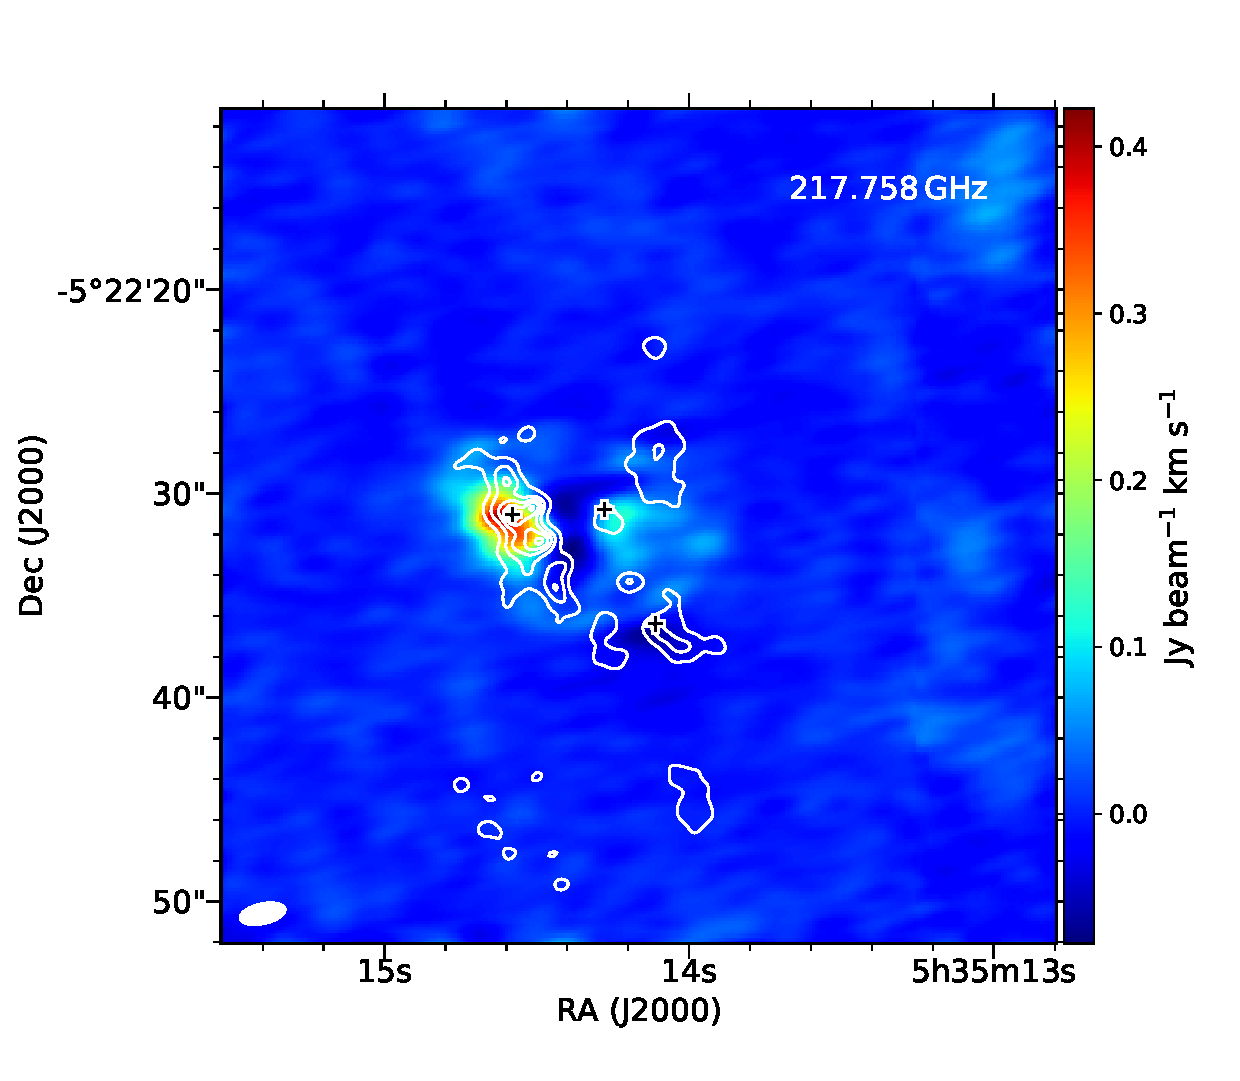
\includegraphics[width=0.98\textwidth]{OrionKL/mom0/217.758mom0_3-7.eps}
%\\(a) 左の図の説明
\end{center}
\end{minipage}
\begin{minipage}{0.48\textwidth}
\begin{center}
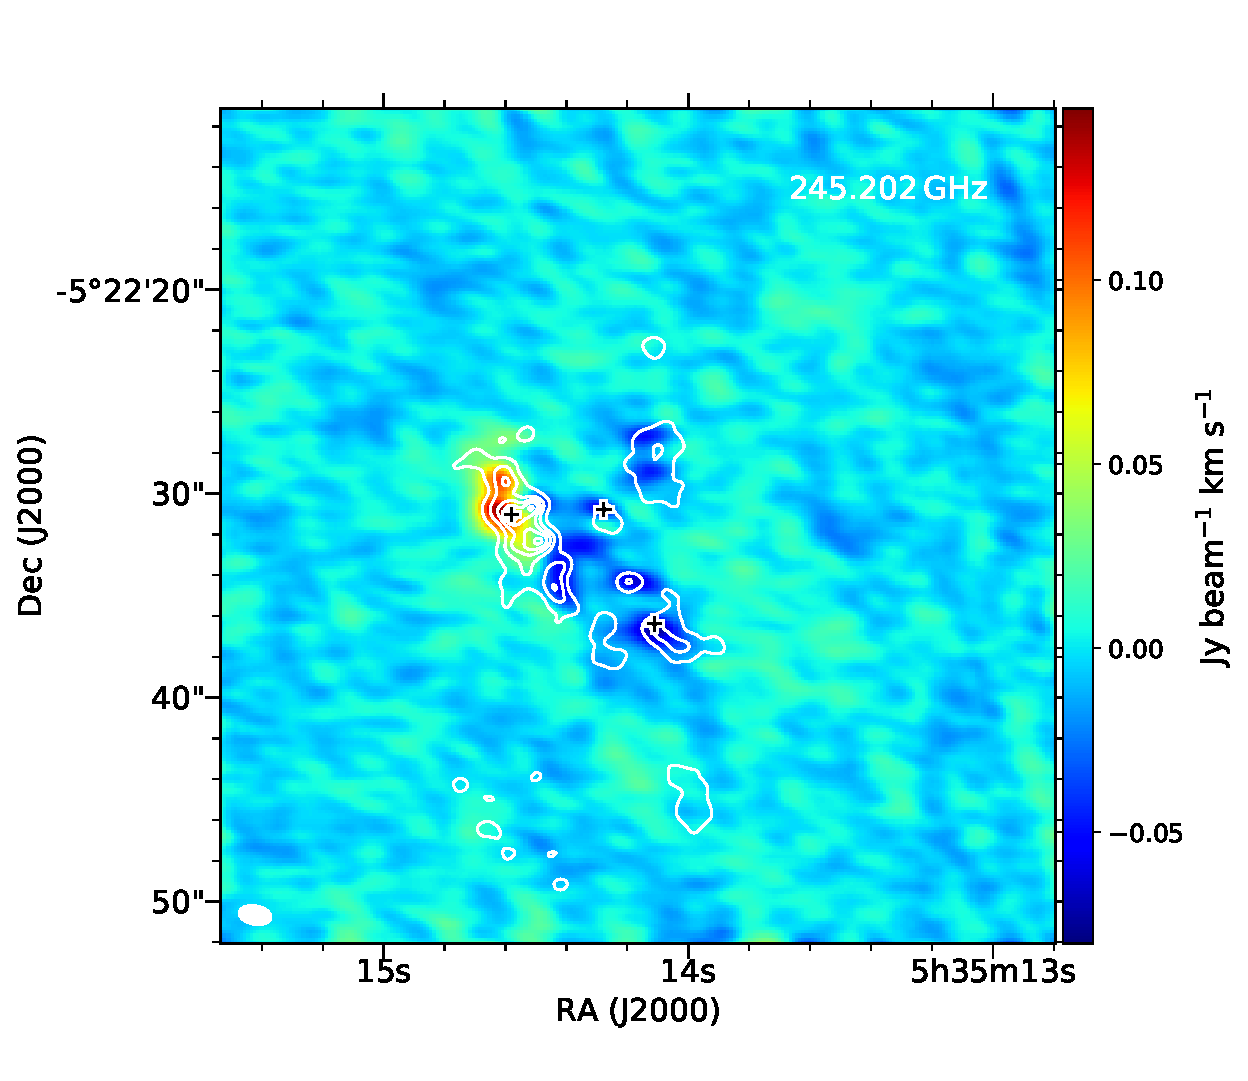
\includegraphics[width=0.98\textwidth]{OrionKL/mom0/245.202mom0_3-7.eps}
%\\(b) 右の図の説明
\end{center}
\end{minipage}
\end{center}
\end{minipage}
%%%% ここまで一組

%\begin{minipage}{0.98\textwidth} 
%\begin{center}
%\begin{minipage}{0.48\textwidth}
%\begin{center}
%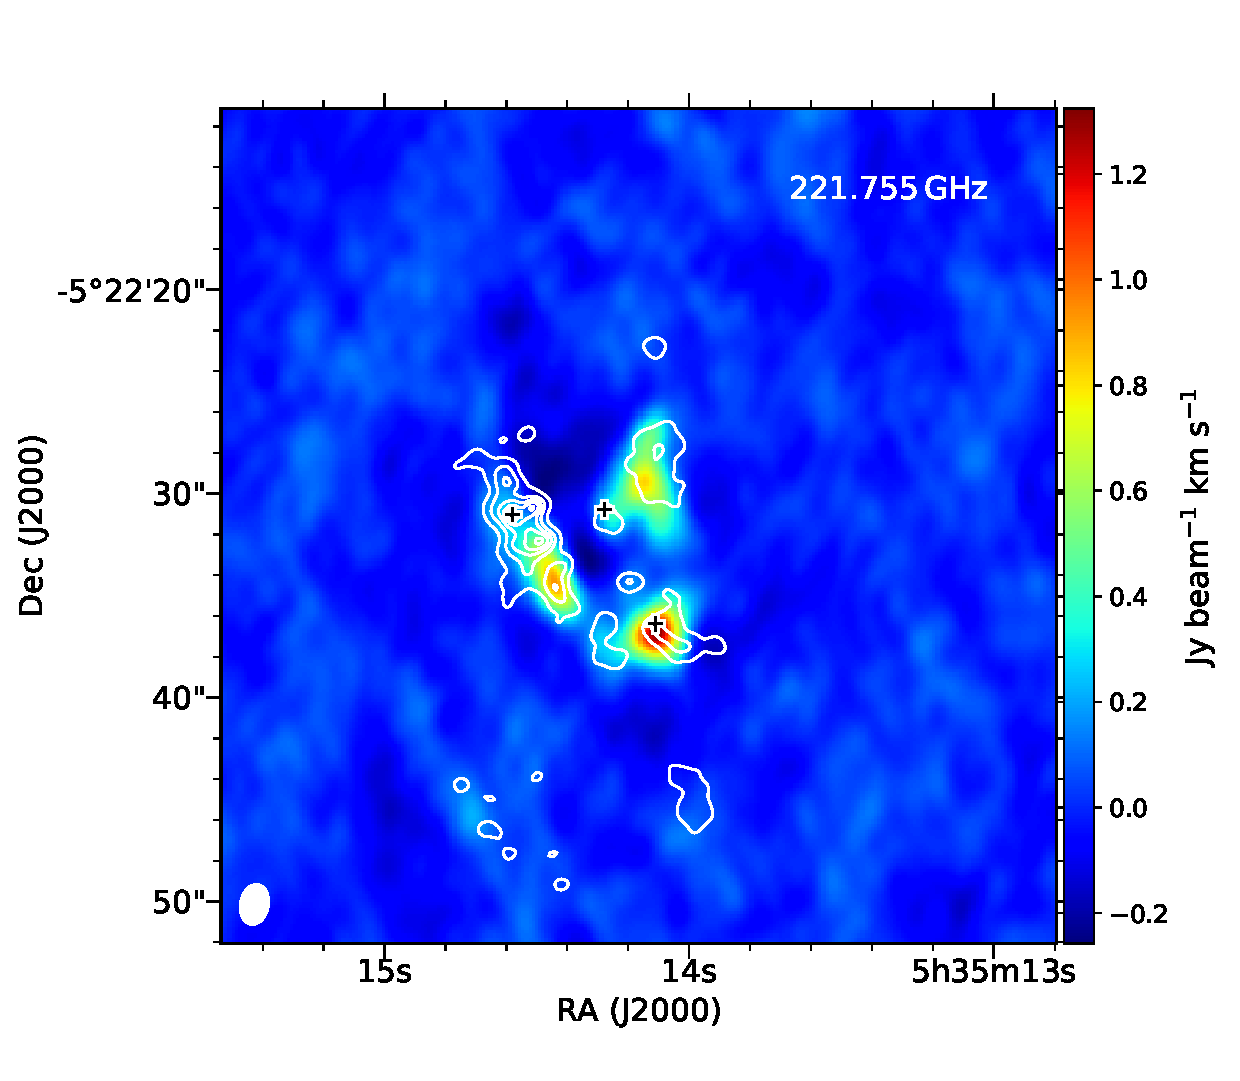
\includegraphics[width=0.98\textwidth]{OrionKL/mom0/221.755SV_mom0_3-7.eps}
%\\(c) 左の図の説明
%\end{center}
%\end{minipage}
%\begin{minipage}{0.48\textwidth}
%\begin{center}
%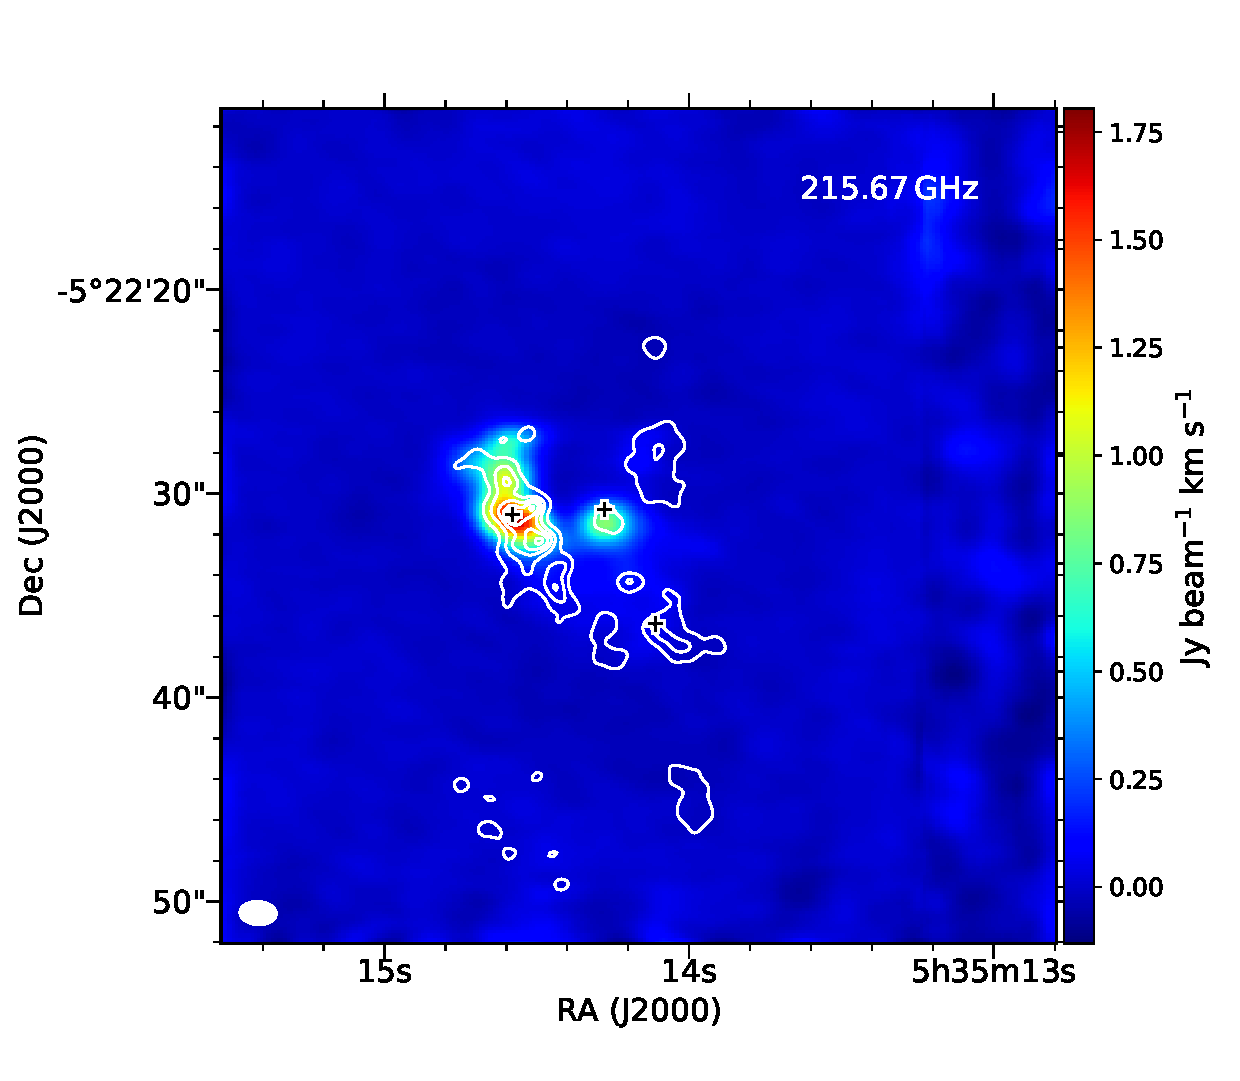
\includegraphics[width=0.98\textwidth]{OrionKL/mom0/215.67mom0_3-7.eps}
%\\(d) 右の図の説明
%\end{center}
%\end{minipage}
%\end{center}
%\end{minipage}
%\end{center}
%\end{figure}

%\begin{figure}[H] 
%\begin{center}
\begin{minipage}{0.98\textwidth} 
\begin{center}
%%%% ここから
\begin{minipage}{0.48\textwidth}
\begin{center}
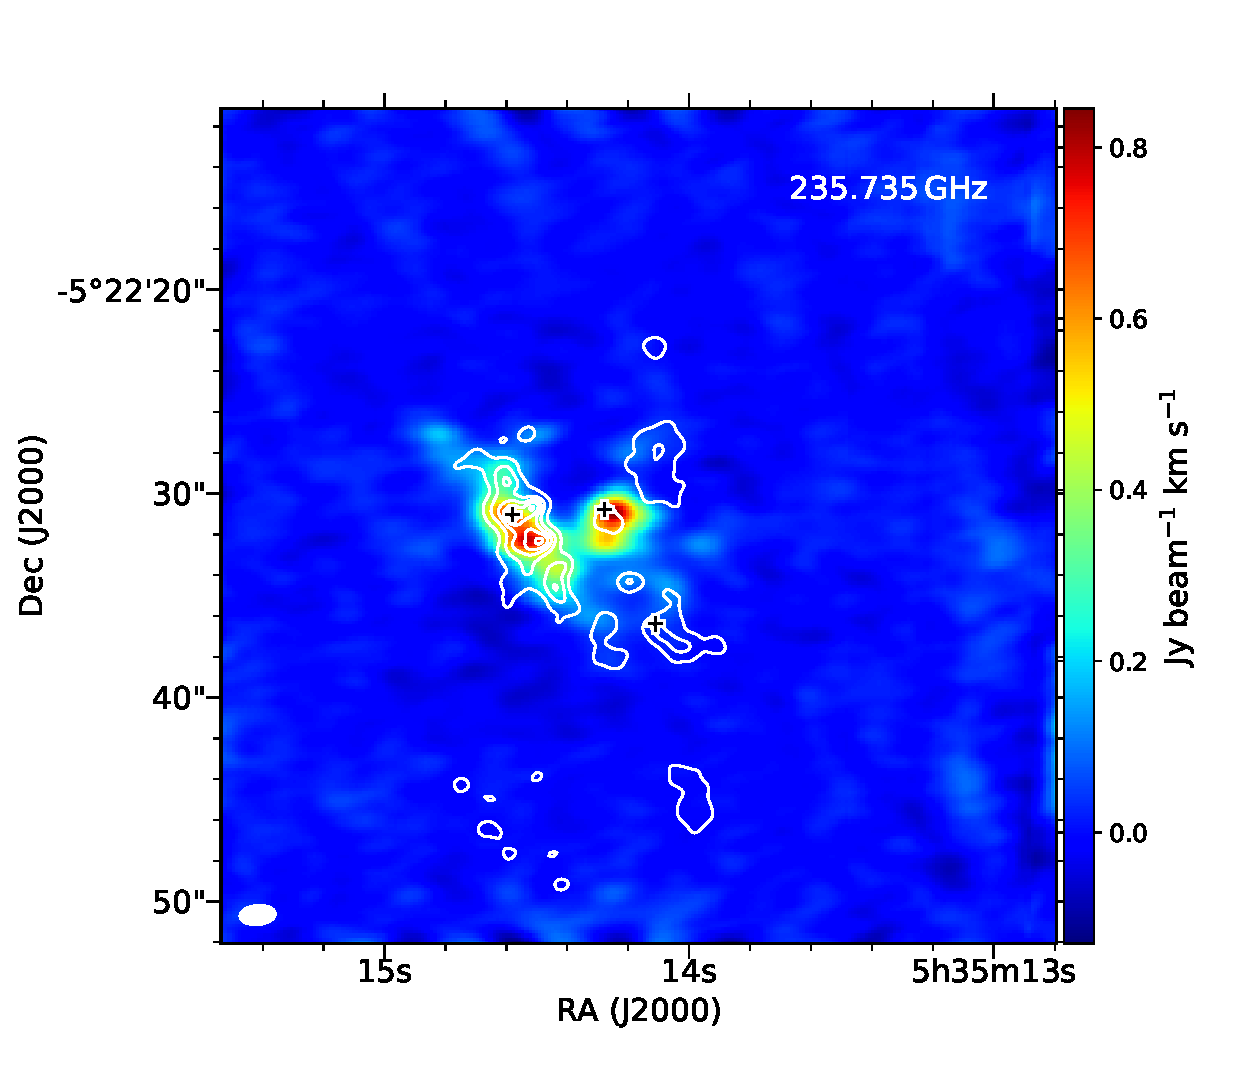
\includegraphics[width=0.98\textwidth]{OrionKL/mom0/235.735mom0_3-7.eps}
%\\(e) 左の図の説明
\end{center}
\end{minipage}
\begin{minipage}{0.48\textwidth}
\begin{center}
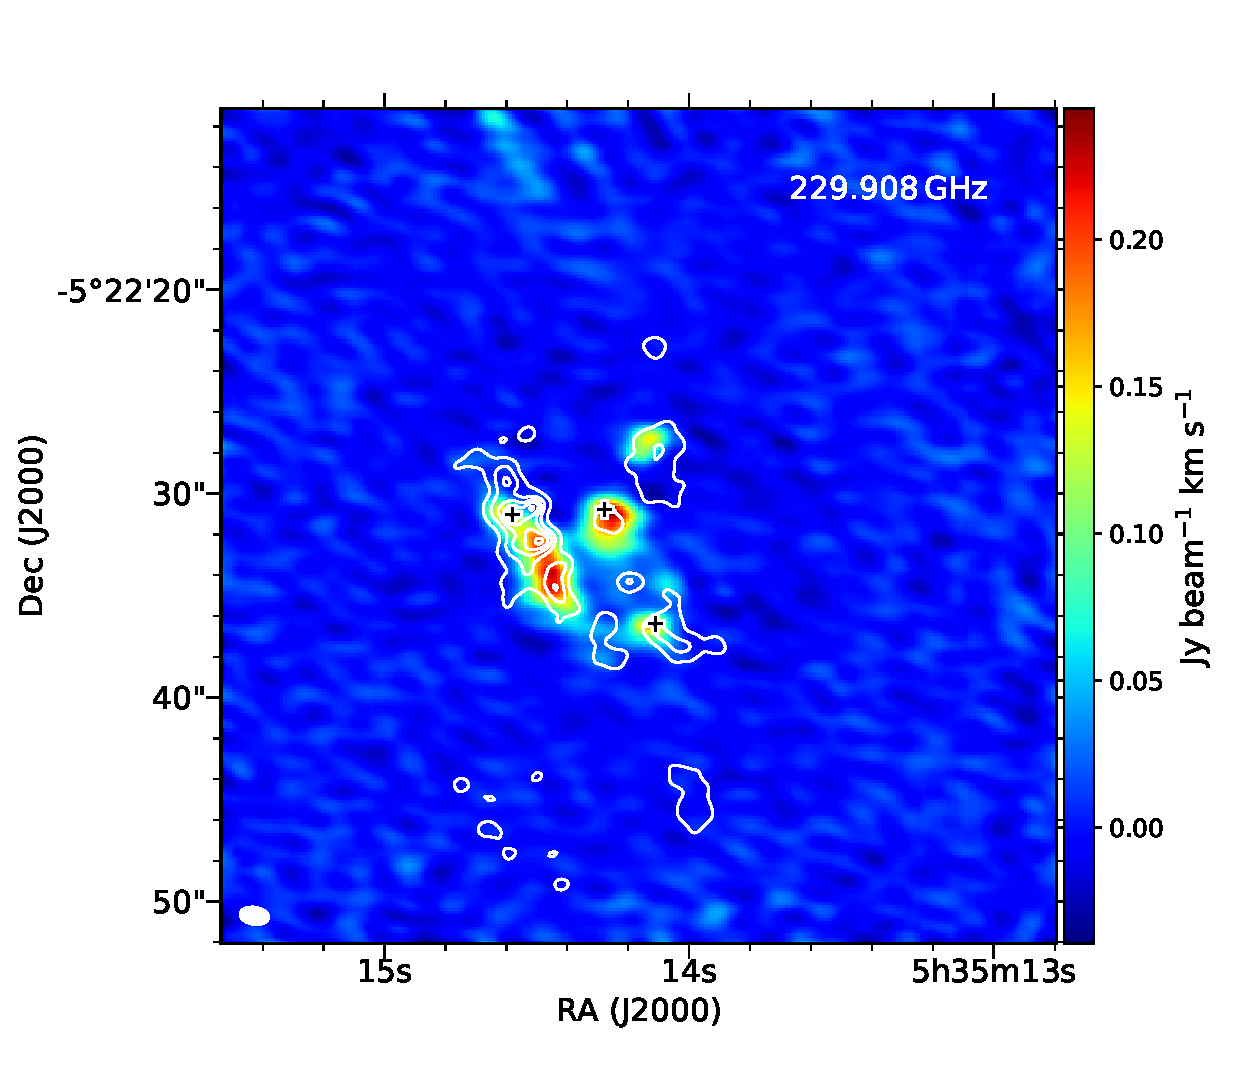
\includegraphics[width=0.98\textwidth]{OrionKL/mom0/229.908mom0_3-7.eps}
%\\(f) 右の図の説明
\end{center}
\end{minipage}
\end{center}
\end{minipage}
%%%% ここまで一組

\begin{minipage}{0.98\textwidth} 
\begin{center}
\begin{minipage}{0.48\textwidth}
\begin{center}
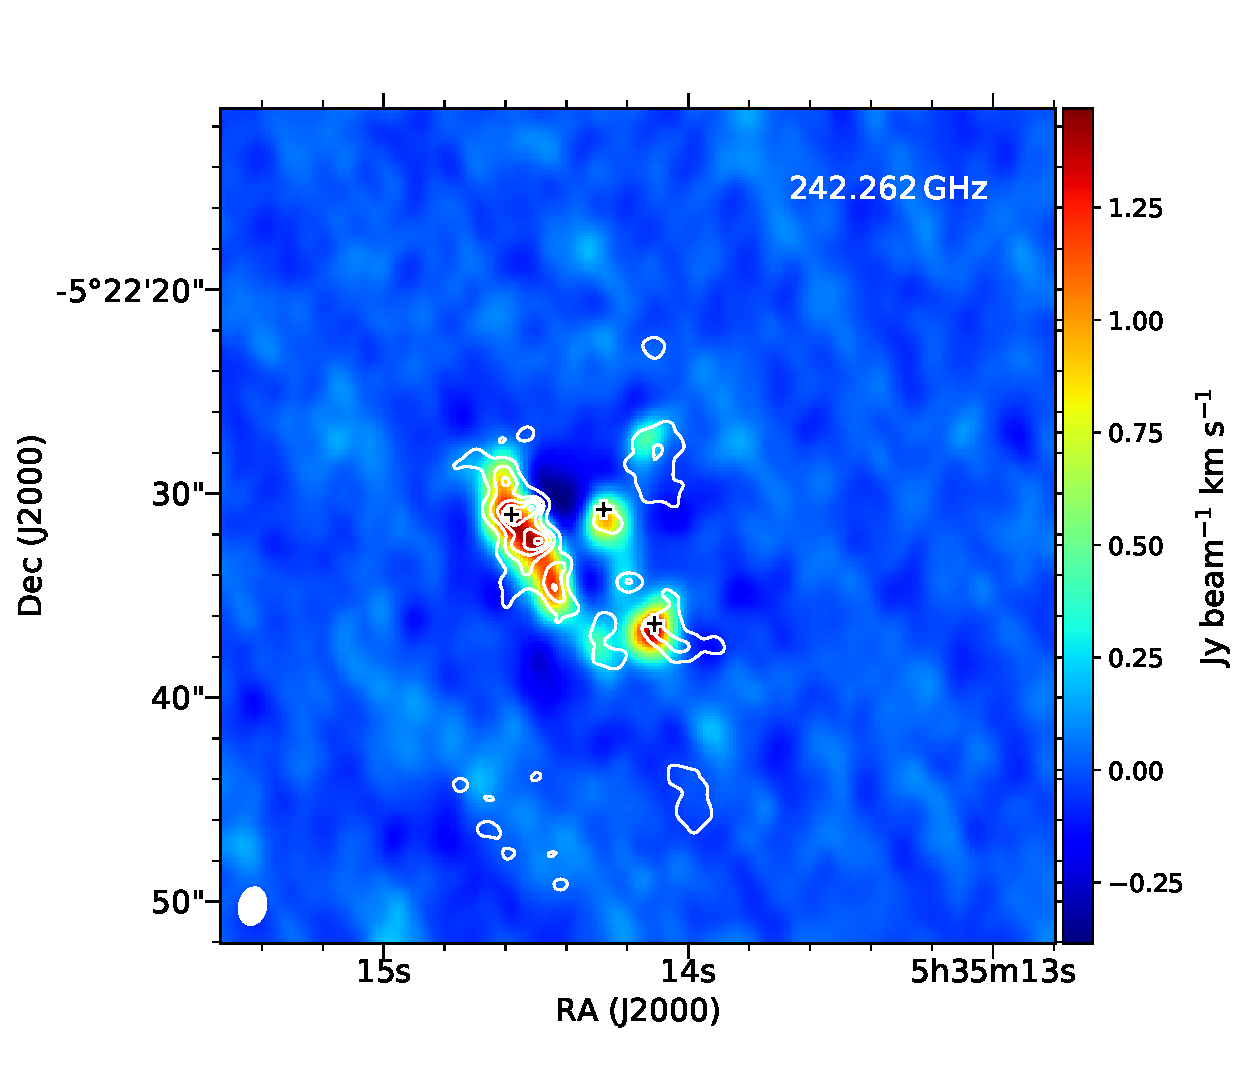
\includegraphics[width=0.98\textwidth]{OrionKL/mom0/242.262SV_mom0_3-7.eps}
%\\(g) 左の図の説明
\end{center}
\end{minipage}
\begin{minipage}{0.48\textwidth}
\begin{center}
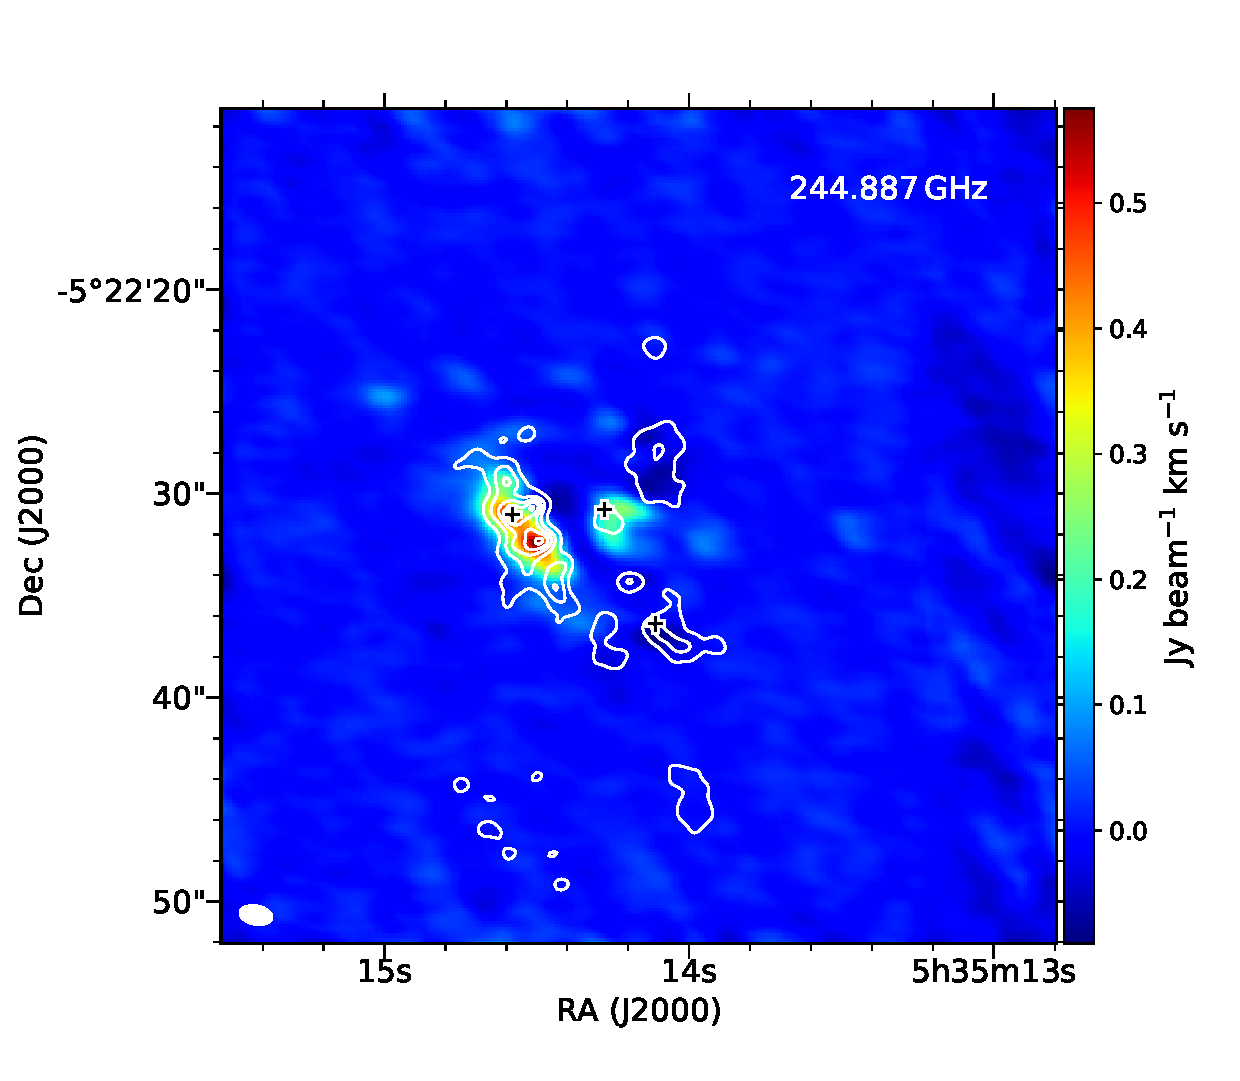
\includegraphics[width=0.98\textwidth]{OrionKL/mom0/244.887mom0_3-7.eps}
%\\(h) 右の図の説明
\end{center}
\end{minipage}
\end{center}
\end{minipage}

\caption{Integrated intensity maps of unblended CH$_{3}$NH$_{2}$ lines. 
The white contours show the 1.3 mm continuum map from \citet{Hirota+2015},
where the contour levels are 10 \%, 30 \%, 50 \%, 70 \%, 90 \% of the peak intensity.
Black crosses denote Hot core, IRc7, and Compact ridge. 
The rest frequency of each transition shows in the upper right part of each panel.}
%\caption{(Continued)}
\end{center}
\end{figure}
%%%%% 積分強度図ここまで %%%%%

%%%%%% チャネルマップここから
\begin{figure}[H]
  \centering
  \includegraphics[width=0.98\textwidth]{OrionKL/chmap/217.758.eps}
  \caption{
  Channel map of expected unblended 217.758 GHz line show multiple velocity-dependent 
  emission peaks: 4-6 km s$^{-1}$ towards Hot core, 7-9km s$^{-1}$ towards IRc7. 
  Magenta crosses denote Hot core, IRc7, and Compact ridge.}
  \label{ch_0}
\end{figure}

\begin{figure}[H]
  \centering
  \includegraphics[width=0.98\textwidth]{OrionKL/chmap/245.202.eps}
  \caption{Channel map of expected unblended 245.202 GHz line.}
  \label{ch_1}
\end{figure}

\begin{figure}[H]
  \centering
  \includegraphics[width=0.98\textwidth]{OrionKL/chmap/235.735.eps}
  \caption{Channel map of expected unblended 235.735 GHz line.}
  \label{ch_2}
\end{figure}

\begin{figure}[H]
  \centering
  \includegraphics[width=0.98\textwidth]{OrionKL/chmap/242.262.eps}
  \caption{Channel map of expected unblended 242.262 GHz line.}
  \label{ch_3}
\end{figure}

\begin{figure}[H]
  \centering
  \includegraphics[width=0.98\textwidth]{OrionKL/chmap/244.887.eps}
  \caption{Channel map of expected unblended 244.887 GHz line.}
  \label{ch_5}
\end{figure}

\begin{figure}[H]
  \centering
  \includegraphics[width=0.98\textwidth]{OrionKL/chmap/229.908.eps}
  \caption{Channel map of expected unblended 229.908 GHz line.}
  \label{ch_7}
\end{figure}

\newpage
\subsection{Spectrum}
The spectrum were extracted from the region of 1''.0 in diameter around 
Hot core (RA$_{J2000}: 05^{\rm{h}}35^{\rm{m}}14^{\rm{s}}.580$, Dec$_{J2000}:-05^{\circ}22'31''.029$), 
and the Gaussian fitting was performed to obtain the line width and Vlsr of the emission line.

%%%%% スペクトル挿入 %%%%%
\begin{figure}[H] 
\begin{center}
\begin{minipage}{0.98\textwidth} 
\begin{center}
%%%% ここから
\begin{minipage}{0.48\textwidth}
\begin{center}
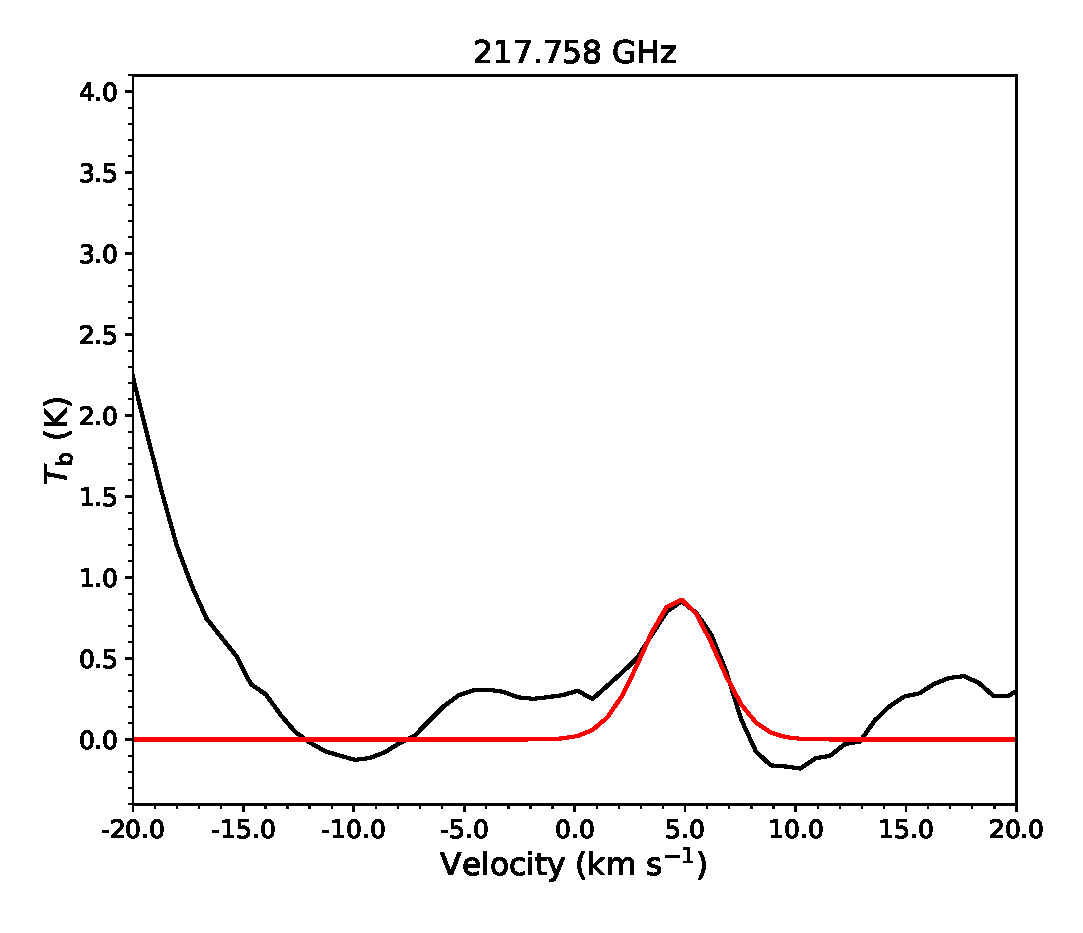
\includegraphics[width=0.98\textwidth]{OrionKL/spectrum/HC/217.758328w_fit.eps}
%\\(a) 左の図の説明
\end{center}
\end{minipage}
\begin{minipage}{0.48\textwidth}
\begin{center}
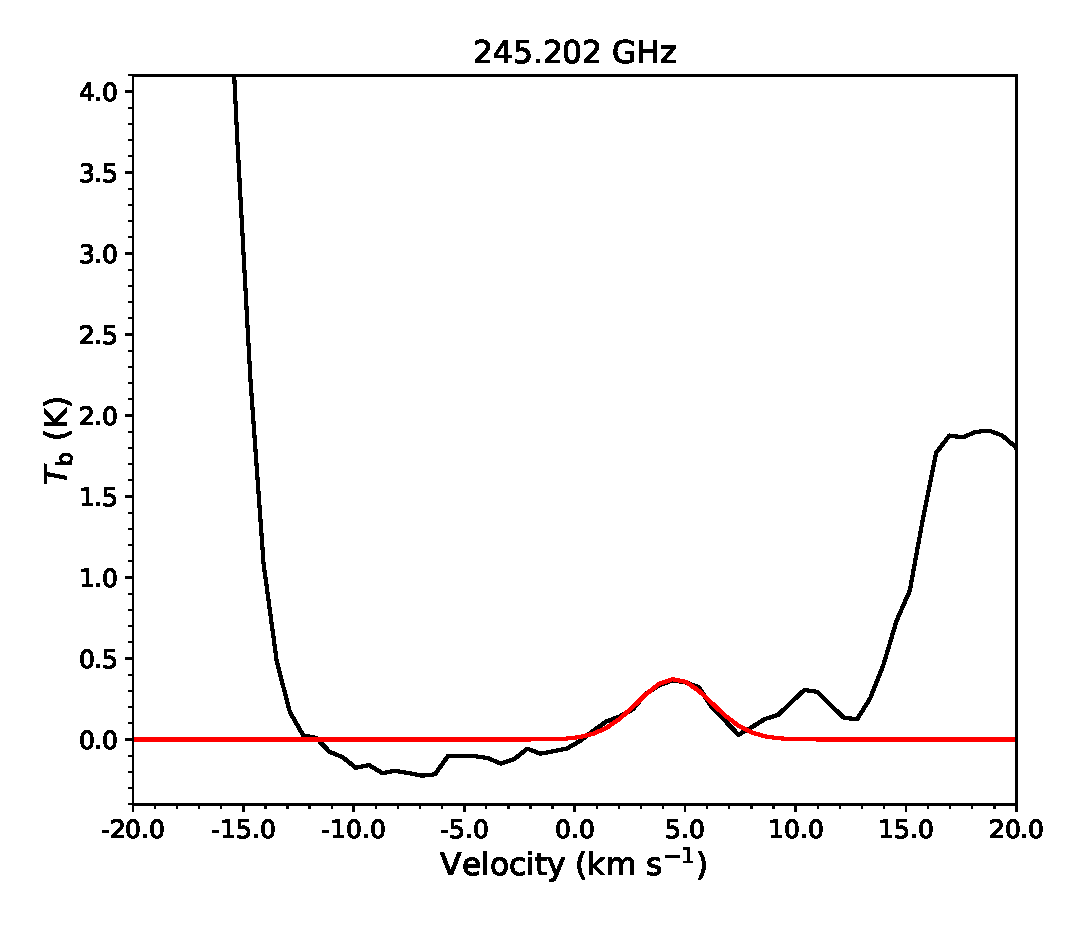
\includegraphics[width=0.98\textwidth]{OrionKL/spectrum/HC/245.2021362w_fit.eps}
%\\(b) 
\end{center}
\end{minipage}
\end{center}
\end{minipage}
%%%% ここまで一組

%\begin{minipage}{0.98\textwidth} 
%\begin{center}
%\begin{minipage}{0.48\textwidth}
%\begin{center}
%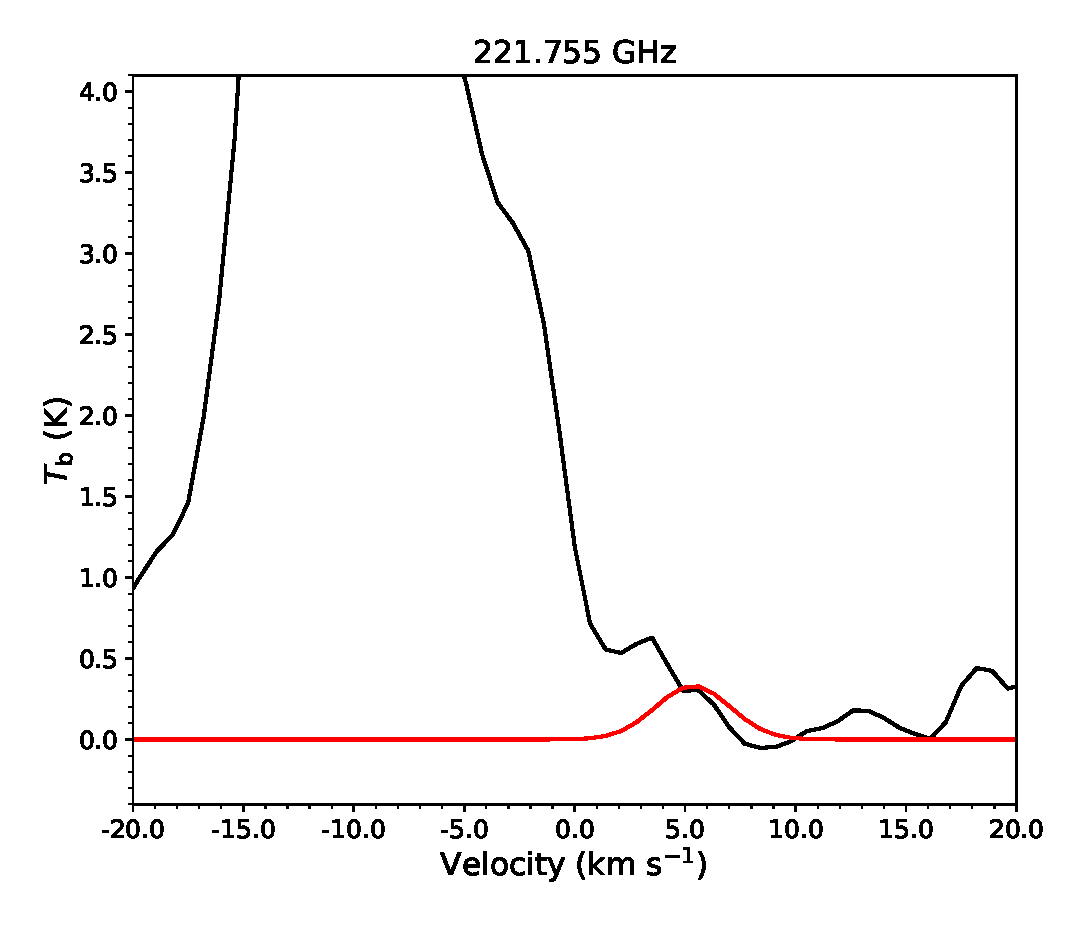
\includegraphics[width=0.98\textwidth]{OrionKL/spectrum/HC/221.755055w_fit.eps}
%\\(c) 左の図の説明
%\end{center}
%\end{minipage}
%\begin{minipage}{0.48\textwidth}
%\begin{center}
%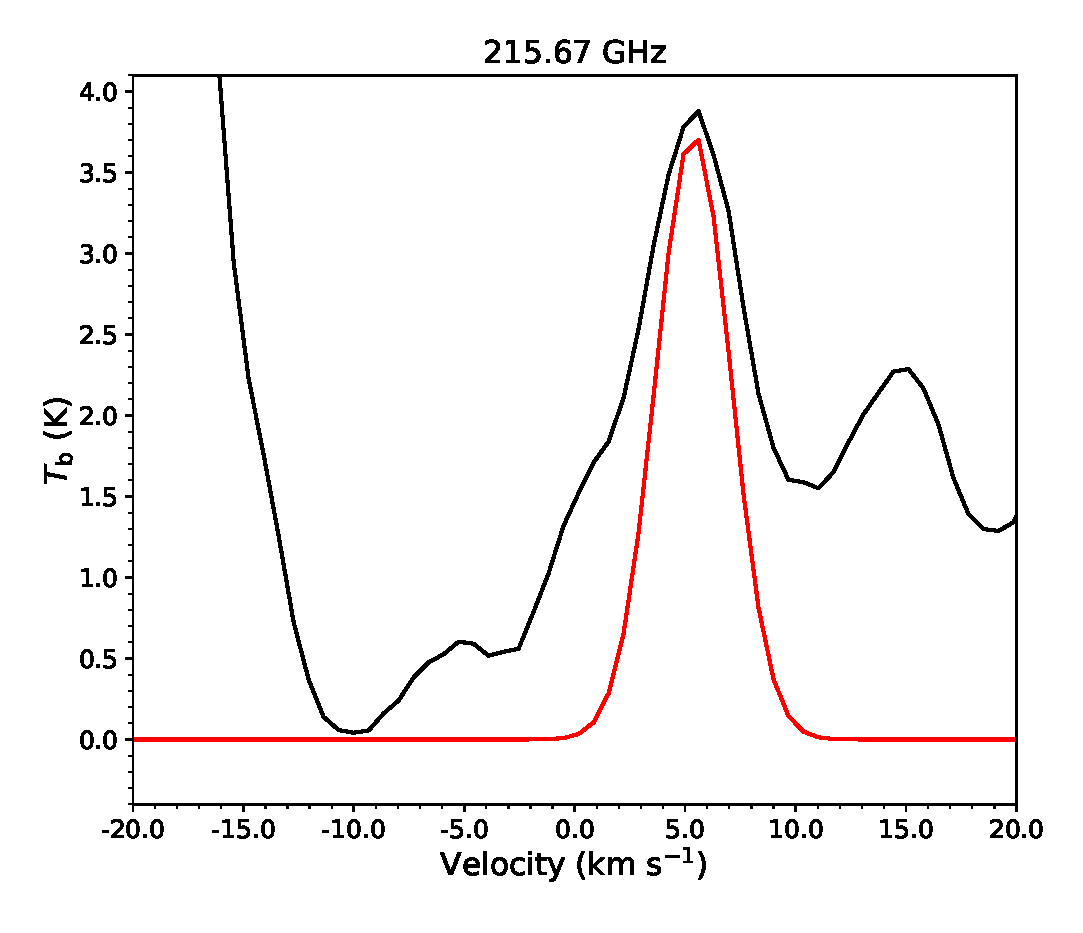
\includegraphics[width=0.98\textwidth]{OrionKL/spectrum/HC/215.6696452w_fit.eps}
%\\(d) 右の図の説明
%\end{center}
%\end{minipage}
%\end{center}
%\end{minipage}
\begin{minipage}{0.98\textwidth} 
\begin{center}
%%%% ここから
\begin{minipage}{0.48\textwidth}
\begin{center}
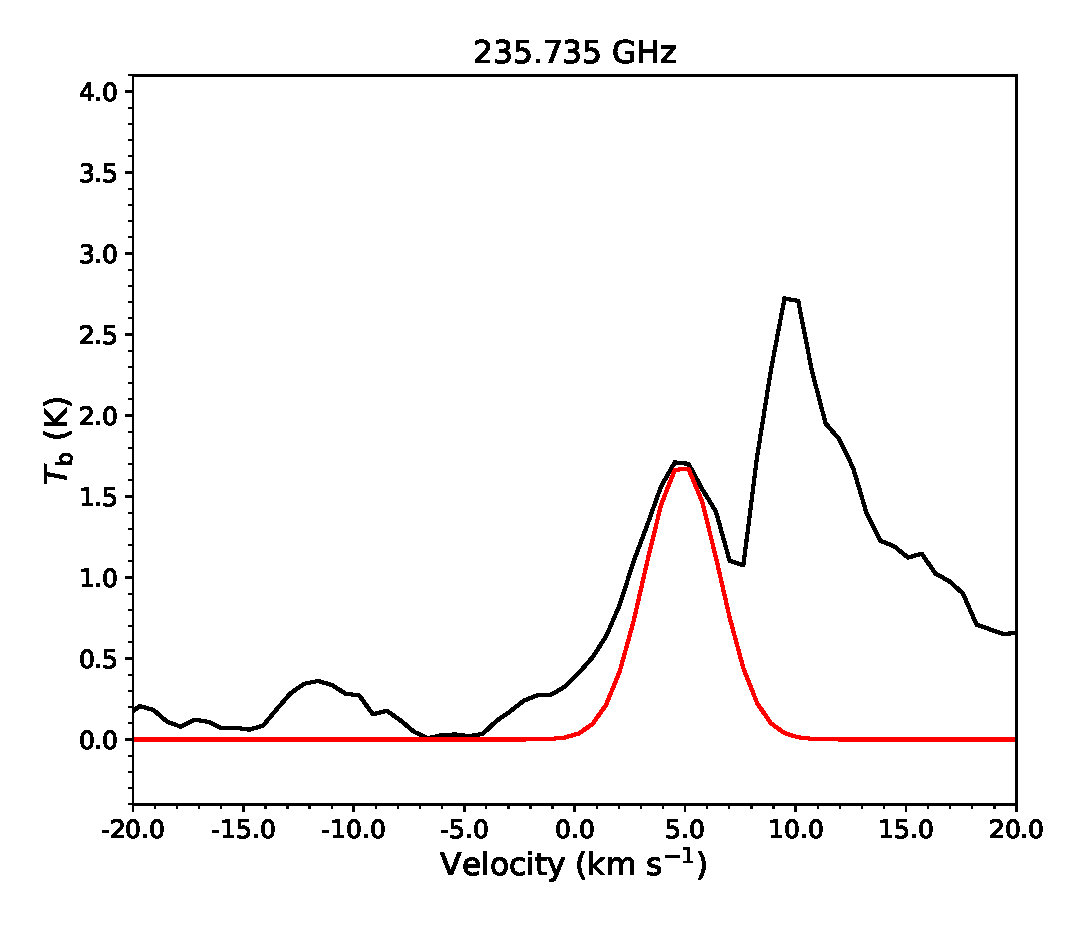
\includegraphics[width=0.98\textwidth]{OrionKL/spectrum/HC/235.735037w_fit.eps}
%\\(e) 左の図の説明
\end{center}
\end{minipage}
\begin{minipage}{0.48\textwidth}
\begin{center}
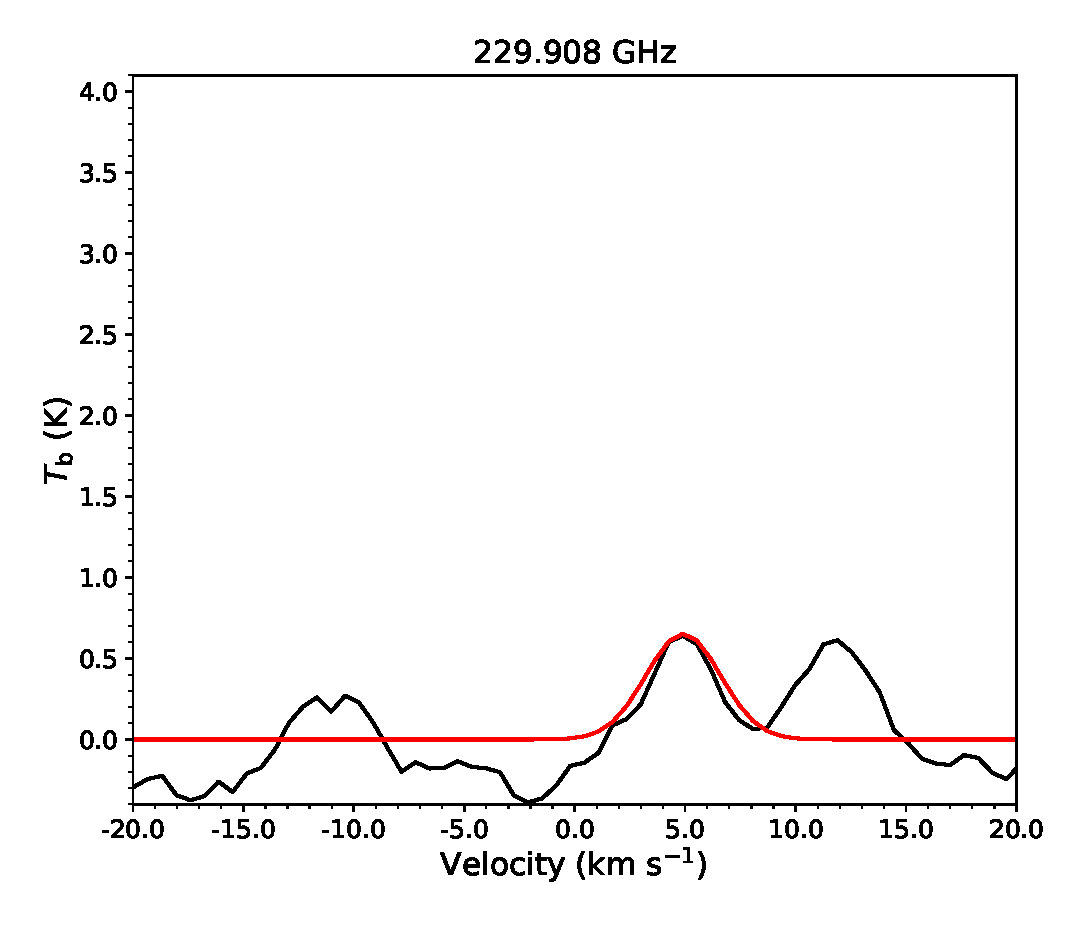
\includegraphics[width=0.98\textwidth]{OrionKL/spectrum/HC/229.908118w_fit.eps}
%\\(f) 右の図の説明
\end{center}
\end{minipage}
\end{center}
\end{minipage}
%%%% ここまで一組

\begin{minipage}{0.98\textwidth} 
\begin{center}
\begin{minipage}{0.48\textwidth}
\begin{center}
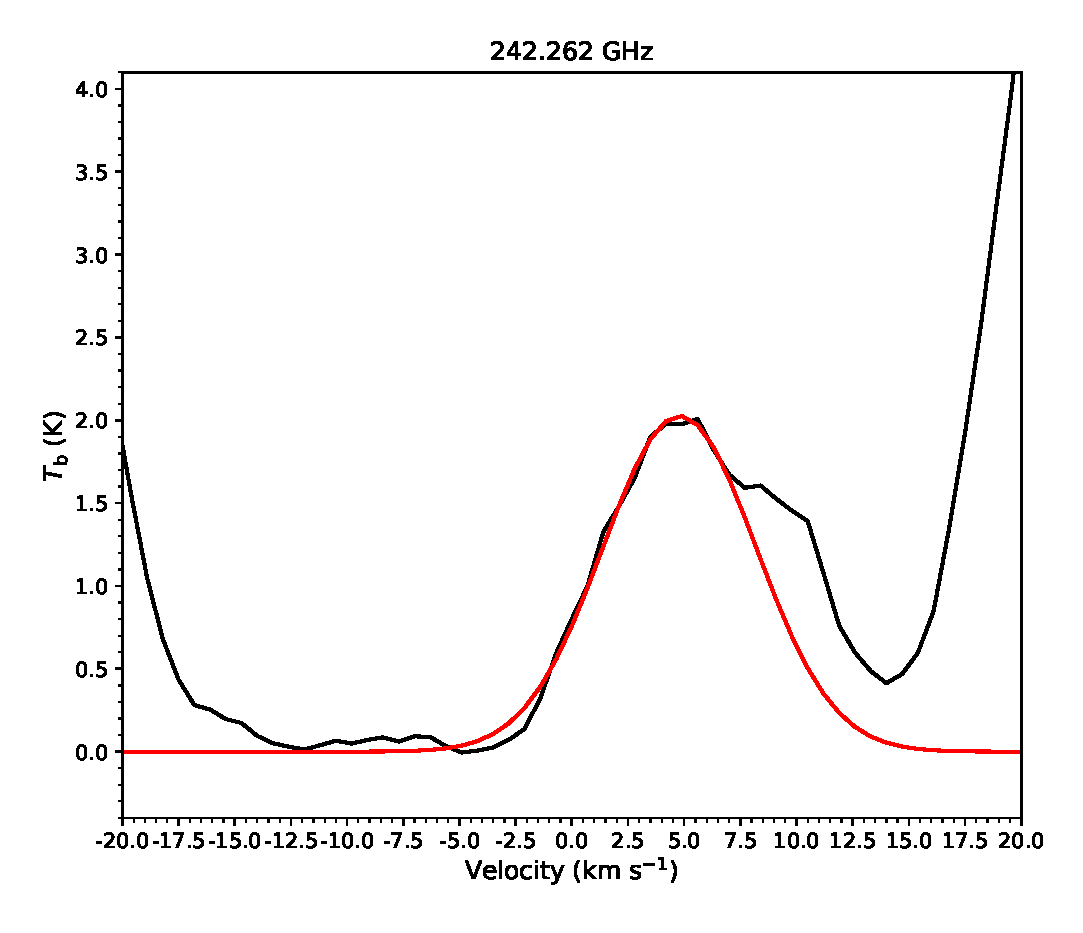
\includegraphics[width=0.98\textwidth]{OrionKL/spectrum/HC/242.2620195w_fit.eps}
%\\(g) 左の図の説明
\end{center}
\end{minipage}
\begin{minipage}{0.48\textwidth}
\begin{center}
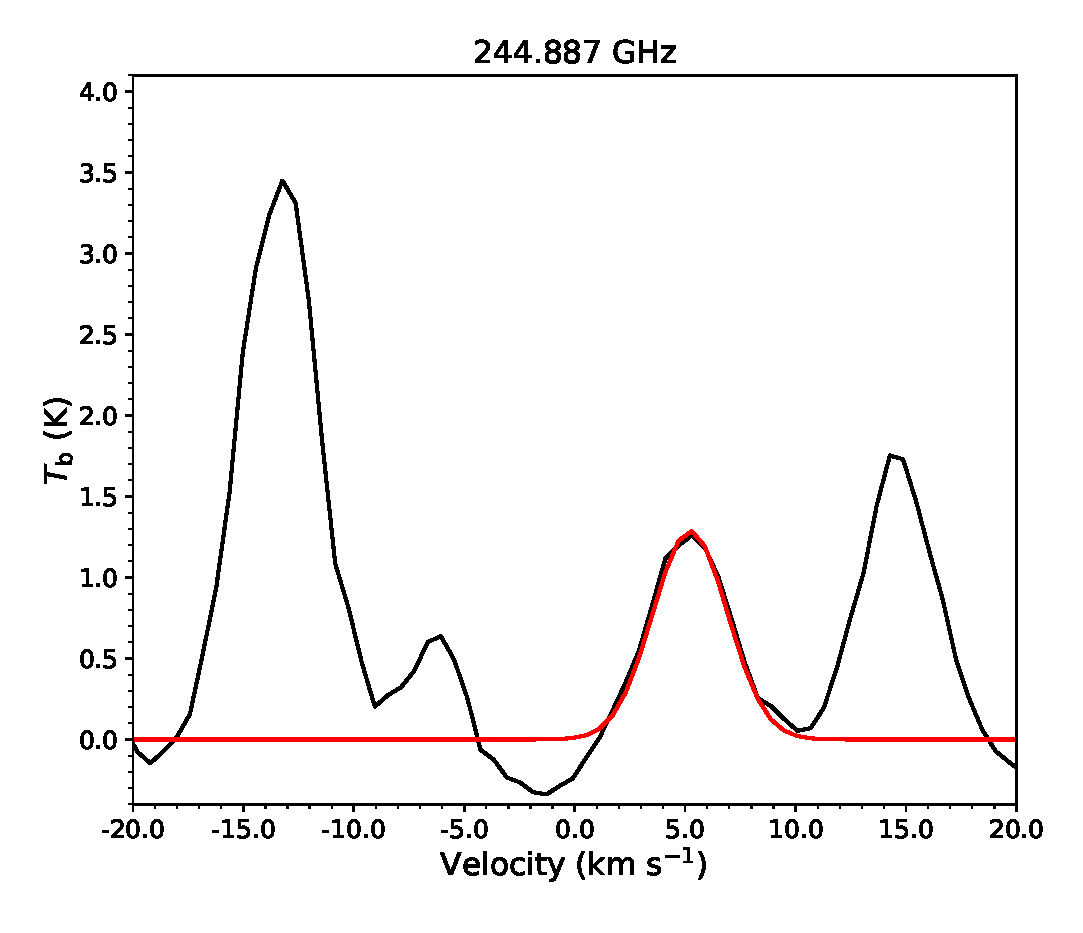
\includegraphics[width=0.98\textwidth]{OrionKL/spectrum/HC/244.8869007w_fit.eps}
%\\(h) 右の図の説明
\end{center}
\end{minipage}
\end{center}
\end{minipage}

\label{fig:spec}
\caption{Spectrum of the CH$_3$NH$_2$ lines at each frequency observed in Hot core center (black) 
  and the result of the Gaussian fitting (red).}
\end{center}
\end{figure}


\section{Disucssion}
\subsection{Column density and Rotation temperature}

In this subsection we will describe the methodologies in deriving fractional abundances of COMs.
The column density of CH$_{3}$NH$_{2}$ ($N_{\mathrm{MA}}$) was established by using 
the rotational temperature diagram method, which assumes local thermodynamic equilibrium 
(LTE) and optically thin emission. 
The following equation was employed for the analysis \citep{Turner1991}:
\begin{align}
\log \dfrac{3\,k_{\mathrm{B}}\,T_{\mathrm{B}} \,\Delta V_{1/2}}{8\, \pi^3\, \nu\, S\, \mu_0^2} = \log \dfrac{N_{\mathrm{MA}}}{U_{\mathrm{rot}}} - \dfrac{E_{\mathrm{u}}}{k_{\mathrm{B}}} \dfrac{\log e}{T_{\mathrm{rot}}}
\label{eq:RD}
\end{align}

In the expression, $\nu$ is the rest frequency of the transition, $\mu_0$ is the permanent dipole moment, 
$U_{\mathrm{rot}}$ is the rotational partition function, $S$ is the line strength, 
$E_{\mathrm{u}}$ is the upper state energy, and $ T_{\mathrm{B}}$ and  $\Delta V_{1/2}$ 
are the brightness temperature and line widths (FWHM, in~km~s$^{-1}$), respectively.
We assumed $\Delta V_{1/2} = 4.0\, \mathrm{km\,s^{-1}}$, which derived by the Gaussian fitting for 
217.758 GHz line.

The brightness temperature can be converted from intensity $I_{\mathrm{\nu}}$
when the Rayleigh-Jeans law is applicable.
\begin{align}
T_{\mathrm{B}} = \dfrac{c^2}{2\,k_{\mathrm{B}}\, \nu^2} \,I_{\mathrm{\nu}}
\end{align}

\begin{figure}[H]
  \centering
  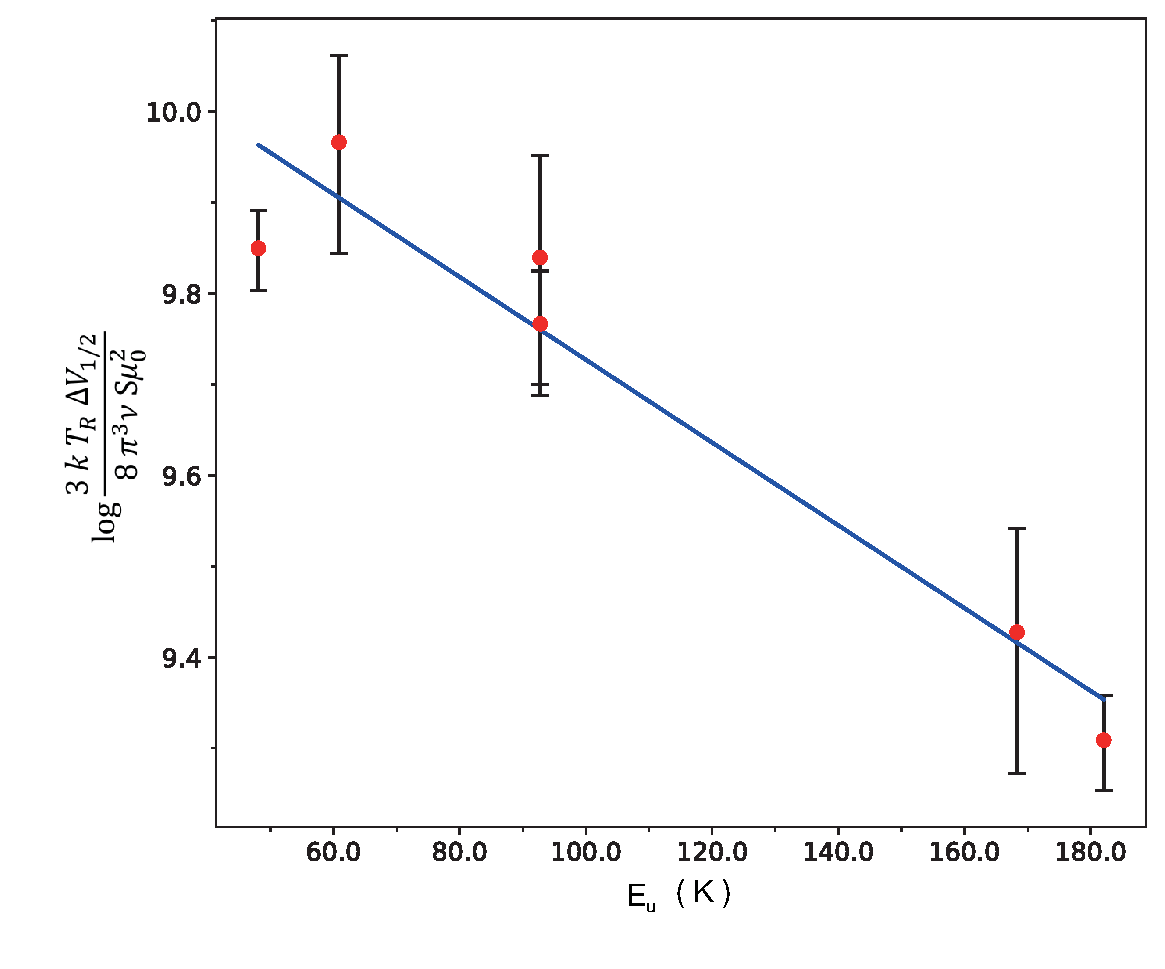
\includegraphics[width=0.8\textwidth]{OrionKL/RD_6point_label.eps}
  \caption{Rotation diagram of CH$_{3}$NH$_{2}$ in Hot core. The error bars represents $\pm$ 3 $\sigma$ for each data.}
  \label{fig:RD}
\end{figure}

The resulting plots are given in Figure \ref{fig:RD}.
The analysis yields a rotational temperature of $T_{\mathrm{rot}} =  95.4^{+15.5}_{-11.7} \,\,\mathrm{K}$, 
with a column density of $N_{\mathrm{MA}} = ( 5.5^{+1.6}_{-1.1} ) \times 10^{14} \,\,\mathrm{cm^{-2}}$.

\subsection{Undetectable lines}
Comparison of catalogs did not suggest contamination, but some emission lines could not be detected as CH$_{3}$NH$_{2}$.

\renewcommand{\arraystretch}{1.5}
\begin{table}[htb]
\begin{center}

  \caption{transitions of CH$_3$NH$_2$}
  \label{tab:unresolved}
{\scriptsize
  \begin{tabular}{cccccccl} \hline
   Fequency [GHz]& S$\mu ^{2}$ [D$^2$] & E$_{\rm{u}}$ [K]& Transition ($J$, $K_{\rm{a}}$, $\Gamma$) 
   & peak $T_{\mathrm{B}}$ [K] & $V_{\mathrm{LSR}}$ [km s$^{-1}$] & Noise [K]  &Comments \\ \hline 
    215.670 & 53.92 & 111.48 & 9, 2, $E_{1-1}$ $\rightarrow$ 9, 1, $E_{1+1}$  & 3.74(0.07) & 5.37(0.07) & 0.043 &  \\
    221.755 & 35.06 & 133.11 & 10, 2, $A_{2}$ $\rightarrow$ 10, 1, $A_{1}$ & 0.33(0.03)& 5.35(0.19) & 0.133 &SV data \\ \hline
  \end{tabular}
  }
\end{center}
\end{table}

As shown in Figure \ref{fig:RD_7point}, the CH$_{3}$NH$_{2}$ data including 2 transitions in Table \ref{tab:unresolved} 
produced point-to-point scatter perhaps because of the lower signal-to-noise ratio for the weaker transitions in SV data 
and possible low-level contamination.

\begin{figure}[H]
  \centering
  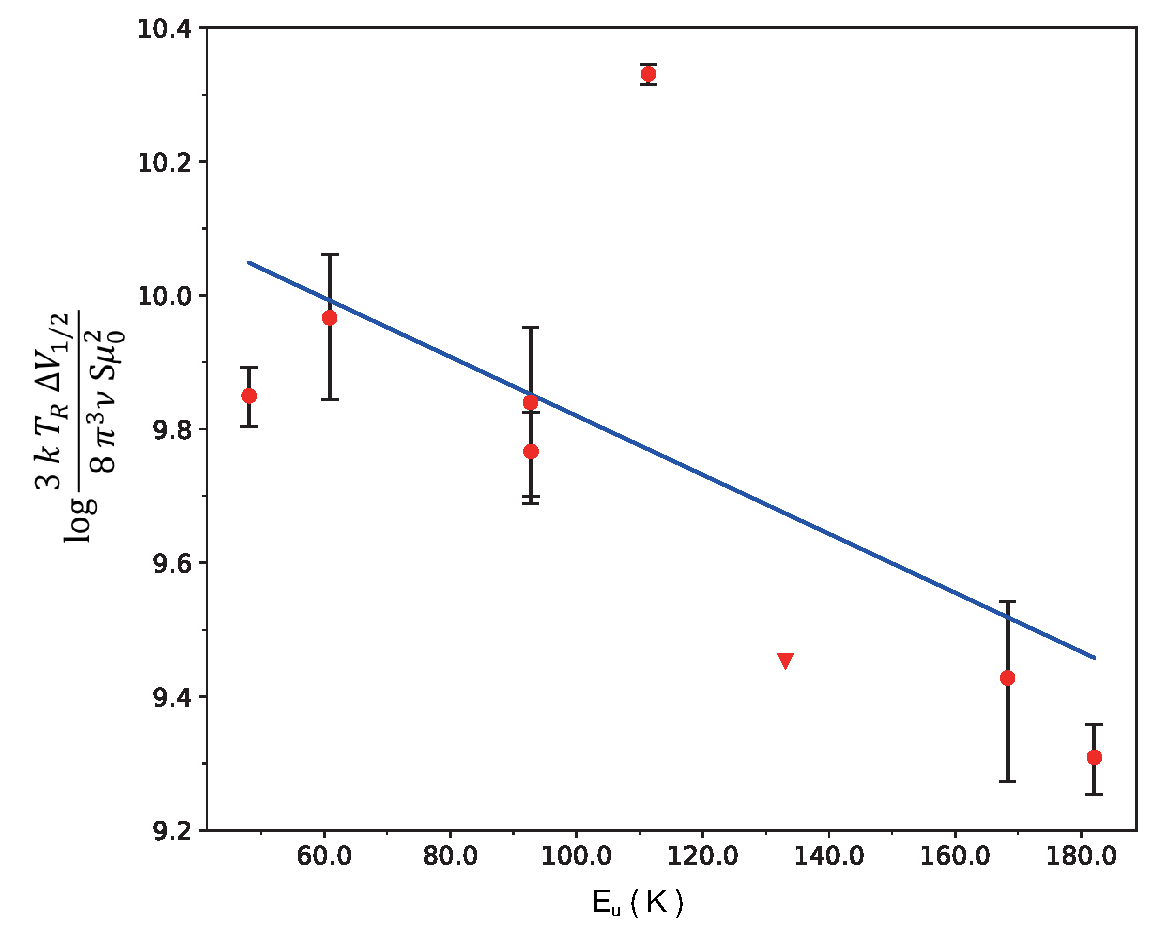
\includegraphics[width=0.7\textwidth]{OrionKL/RD_7point_label.eps}
  \caption{Rotation diagram of CH$_{3}$NH$_{2}$ in Hot core with more 2 lines. The error bars represents $\pm$ 3 $\sigma$ for each data. Upper limit is indicated with triangle. ※6点のみ用いた一次関数と、ノイズレベルの上限も含めた図に差し替え }
  \label{fig:RD_7point}
\end{figure}

\subsubsection*{215.670 GHz line}

\begin{figure}[H] 
\begin{center}
\begin{minipage}{0.98\textwidth} 
\begin{center}
\begin{minipage}{0.48\textwidth}
\begin{center}
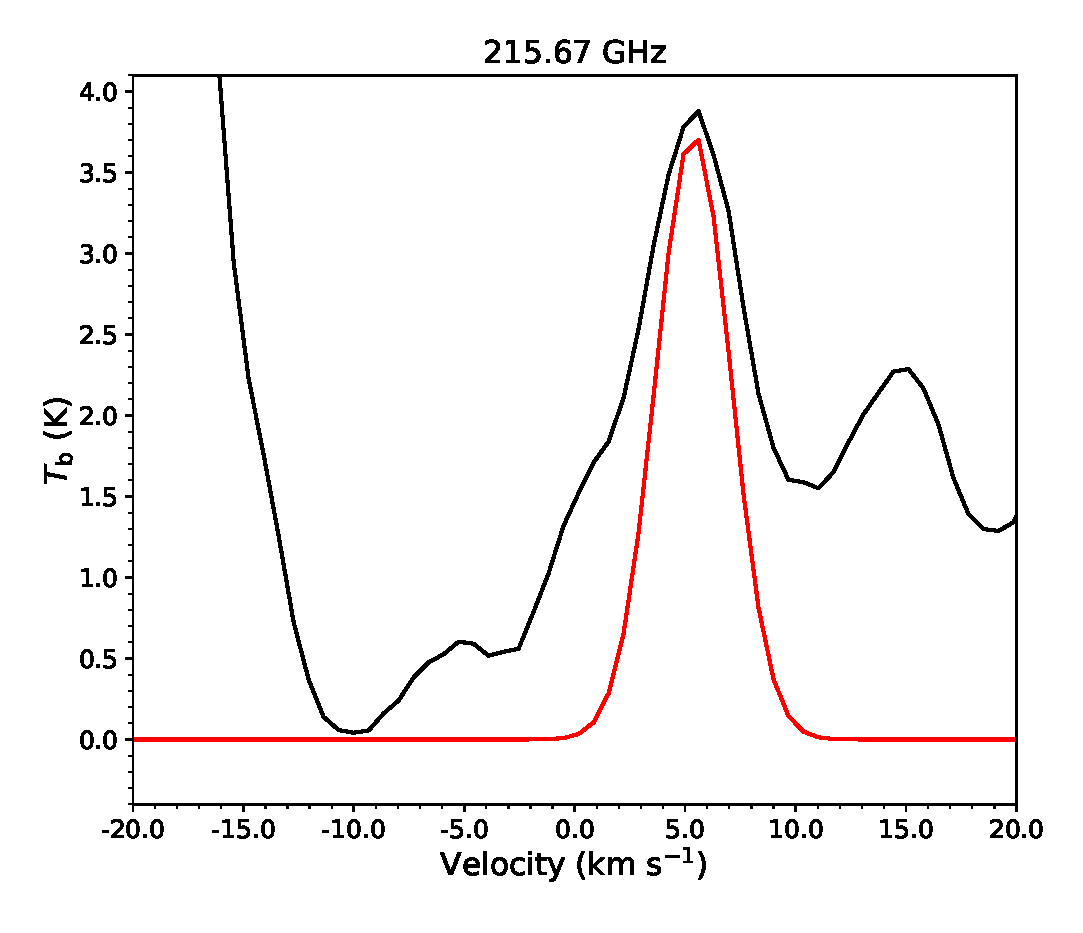
\includegraphics[width=0.98\textwidth]{OrionKL/spectrum/HC/215.6696452w_fit.eps}
\\(c) 左の図の説明
\end{center}
\end{minipage}
\begin{minipage}{0.48\textwidth}
\begin{center}
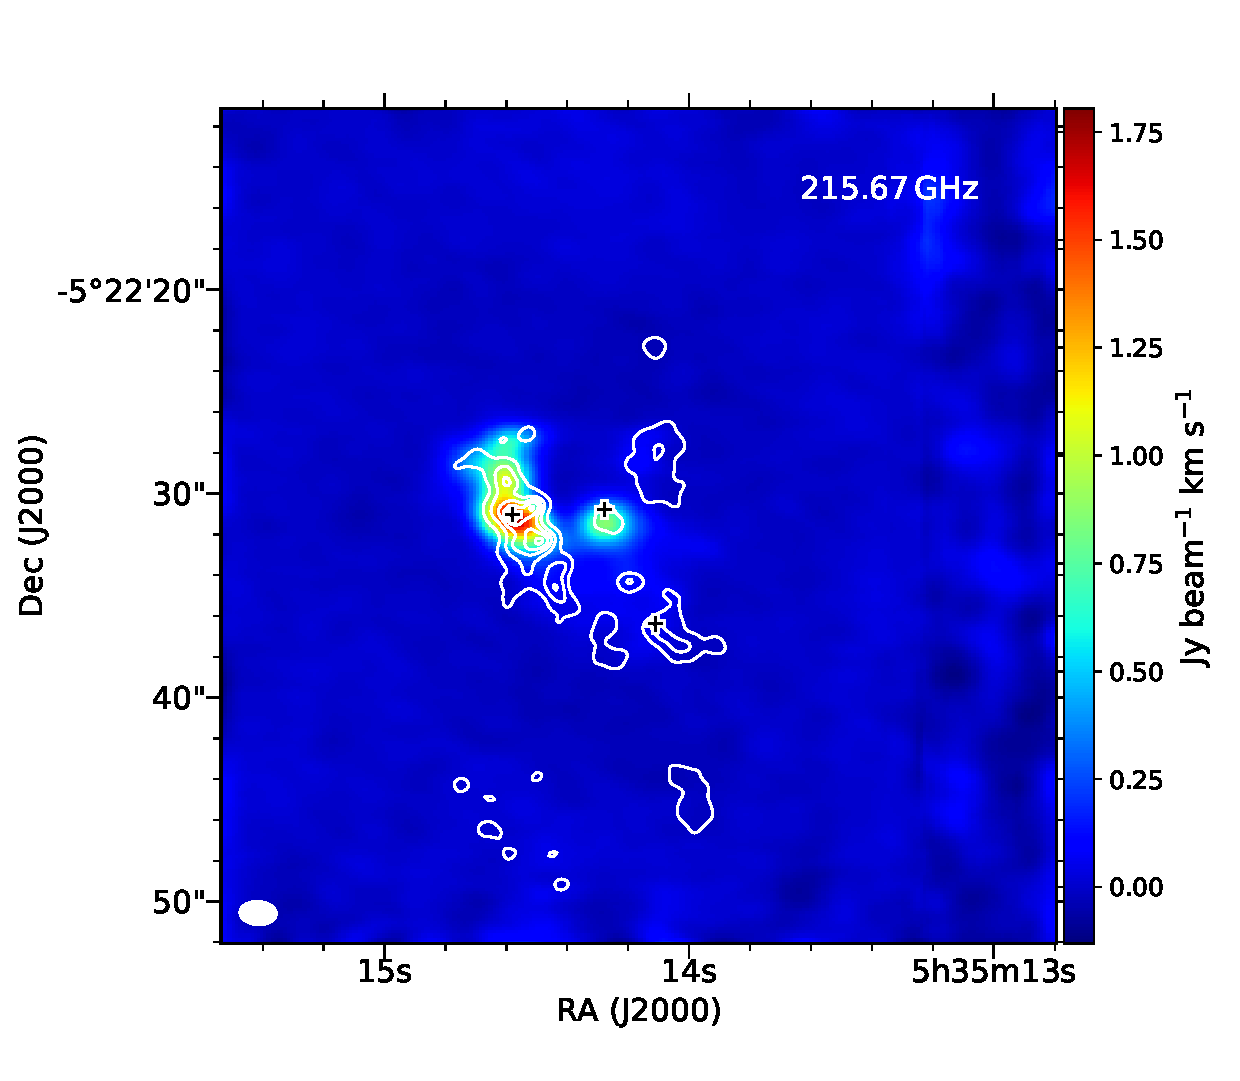
\includegraphics[width=0.98\textwidth]{OrionKL/mom0/215.67mom0_3-7.eps}
\\(d) 右の図の説明
\end{center}
\end{minipage}
\end{center}
\end{minipage}
\caption{215GHz.}
\end{center}
\end{figure}

\begin{figure}[H]
  \centering
  \includegraphics[width=0.98\textwidth]{OrionKL/chmap/215.67.eps}
  \caption{Channel map of expected unblended 215.670 GHz line.}
  \label{ch_4}
\end{figure}

\subsubsection*{221.755 GHz line}

\begin{figure}[H] 
\begin{center}
\begin{minipage}{0.98\textwidth} 
\begin{center}
\begin{minipage}{0.48\textwidth}
\begin{center}
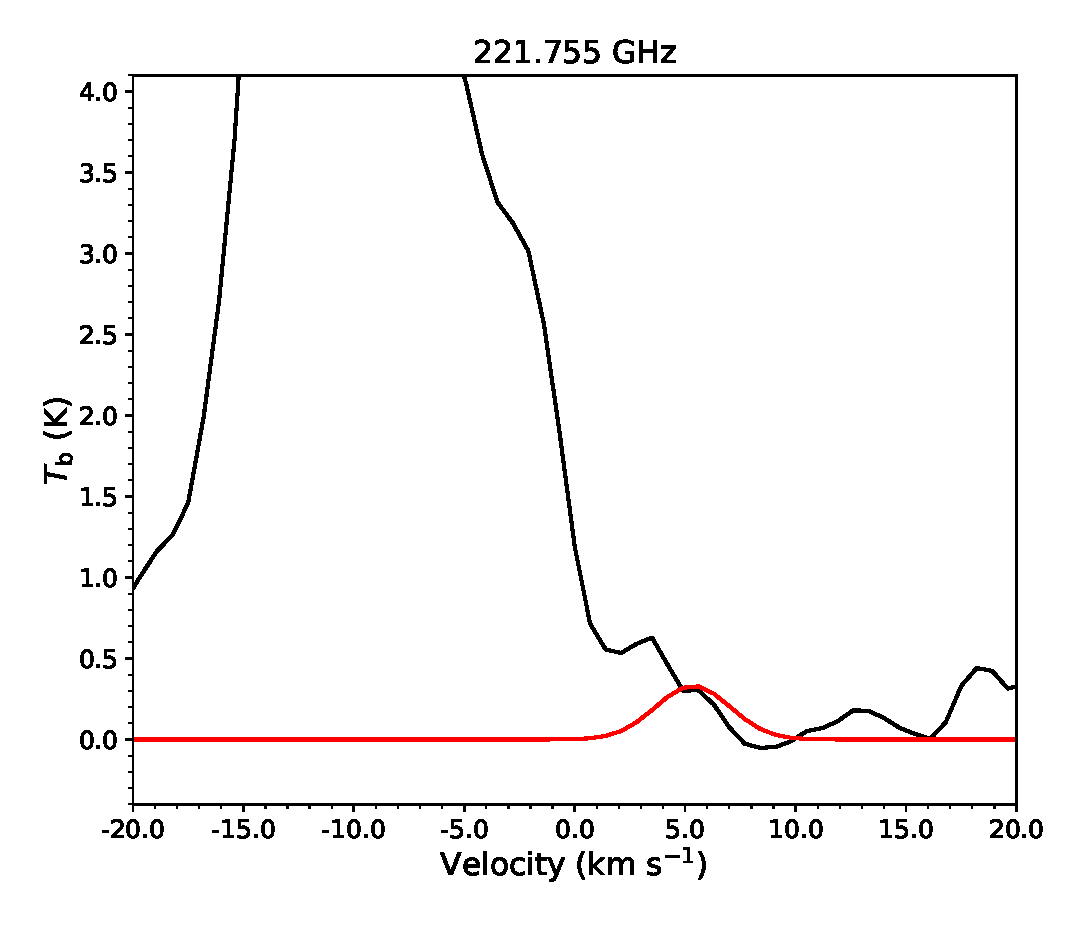
\includegraphics[width=0.98\textwidth]{OrionKL/spectrum/HC/221.755055w_fit.eps}
\\(c) 左の図の説明
\end{center}
\end{minipage}
\begin{minipage}{0.48\textwidth}
\begin{center}
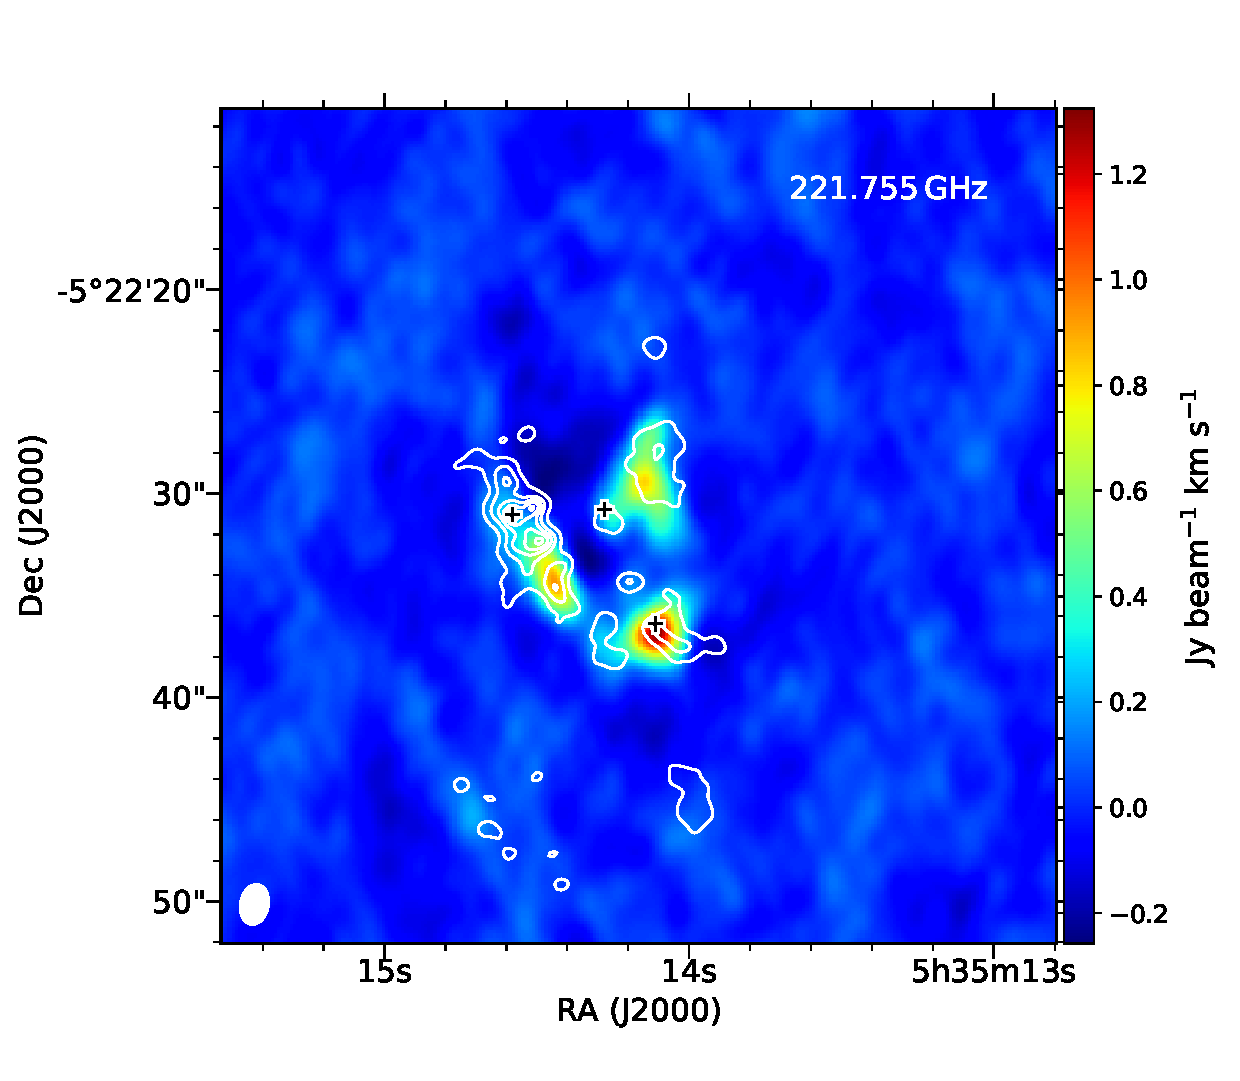
\includegraphics[width=0.98\textwidth]{OrionKL/mom0/221.755SV_mom0_3-7.eps}
\\(d) 右の図の説明
\end{center}
\end{minipage}
\end{center}
\end{minipage}
\caption{221.755 GHz.}
\end{center}
\end{figure}

\begin{figure}[H]
  \centering
  \includegraphics[width=0.98\textwidth]{OrionKL/chmap/221.755.eps}
  \caption{Channel map of expected unblended 221.755 GHz line.}
  \label{ch_6}
\end{figure}
